%\documentclass[../KlassMech_main.tex]{subfiles}
\documentclass[ngerman, DIV=11, BCOR=0mm, paper=a4, fontsize=11pt, parskip=half, twoside=false, titlepage=true]{scrreprt}
%\graphicspath{ {Bilder/} {../Bilder/} }


\usepackage[singlespacing]{setspace}
\usepackage{lastpage}
\usepackage[automark, headsepline]{scrlayer-scrpage}
\clearscrheadings
\setlength{\headheight}{\baselineskip}
%\automark[part]{section}
\automark[chapter]{chapter}
\automark*[chapter]{section} %mithilfe des * wird nur ergänzt; bei vorhandener section soll also das in der Kopfzeile stehen
\automark*[chapter]{subsection}
\ihead[]{\headmark}
%\ohead[]{Seite~\thepage}
\cfoot{\hypersetup{linkcolor=black}Seite~\thepage~von~\pageref{LastPage}}

\usepackage[utf8]{inputenc}
\usepackage[ngerman, english]{babel}
\usepackage[expansion=true, protrusion=true]{microtype}
\usepackage{amsmath}
\usepackage{amsfonts}
\usepackage{amsthm}
\usepackage{amssymb}
\usepackage{mathtools}
\usepackage{mathdots}
\usepackage{aligned-overset} % otherwise, overset/underset shift alignment
\usepackage{upgreek}
\usepackage[free-standing-units]{siunitx}
\usepackage{esvect}
\usepackage{graphicx}
\usepackage{epstopdf}
\usepackage[hypcap]{caption}
\usepackage{booktabs}
\usepackage{flafter}
\usepackage[section]{placeins}
\usepackage{pdfpages}
\usepackage{textcomp}
\usepackage{subfig}
\usepackage[italicdiff]{physics}
\usepackage{xparse}
\usepackage{wrapfig}
\usepackage{color}
\usepackage{multirow}
\usepackage{dsfont}
\numberwithin{equation}{chapter}%{section}
\numberwithin{figure}{chapter}%{section}
\numberwithin{table}{chapter}%{section}
\usepackage{empheq}
\usepackage{tikz-cd}%für Kommutationsdiagramme
\usepackage{tikz}
\usepackage{pgfplots}
\usepackage{mdframed}
\usepackage{floatpag} % to have clear pages where figures are
%\usepackage{sidecap} % for caption on side -> not needed in the end
\usepackage{subfiles} % To put chapters into main file

\usepackage{hyperref}
\hypersetup{colorlinks=true, breaklinks=true, citecolor=linkblue, linkcolor=linkblue, menucolor=linkblue, urlcolor=linkblue} %sonst z.B. orange bei linkcolor

\usepackage{imakeidx}%für Erstellen des Index
\usepackage{xifthen}%damit bei \Def{} das Index-Arugment optional gemacht werden kann

\usepackage[printonlyused]{acronym}%withpage -> seems useless here

\usepackage{enumerate} % for custom enumerators

\usepackage{listings} % to input code

\usepackage{csquotes} % to change quotation marks all at once


%\usepackage{tgtermes} % nimmt sogar etwas weniger Platz ein als default font, aber wenn dann nur auf Text anwenden oder?
\usepackage{tgpagella} % traue mich noch nicht ^^ Bzw macht ganze Formatierung kaputt und so sehen Definitionen nicer aus
%\usepackage{euler}%sieht nichtmal soo gut aus und macht Fehler
%\usepackage{mathpazo}%macht iwie überall pagella an...
\usepackage{newtxmath}%etwas zu dick halt im Vergleich dann; wenn dann mit pagella oder überall Times gut

\setkomafont{chapter}{\fontfamily{qpl}\selectfont\Huge}%{\rmfamily\Huge\bfseries}
\setkomafont{chapterentry}{\fontfamily{qpl}\selectfont\large\bfseries}%{\rmfamily\large\bfseries}
\setkomafont{section}{\fontfamily{qpl}\selectfont\Large}%{\rmfamily\Large\bfseries}
%\setkomafont{sectionentry}{\rmfamily\large\bfseries} % man kann anscheinend nur das oberste Element aus toc setzen, hier also chapter
\setkomafont{subsection}{\fontfamily{qpl}\selectfont\large}%{\rmfamily\large}
\setkomafont{paragraph}{\rmfamily}%\bfseries\itshape}%\underline
\setkomafont{title}{\fontfamily{qpl}\selectfont\Huge\bfseries}%{\Huge\bfseries}
\setkomafont{subtitle}{\fontfamily{qpl}\selectfont\LARGE\scshape}%{\LARGE\scshape}
\setkomafont{author}{\Large\slshape}
\setkomafont{date}{\large\slshape}
\setkomafont{pagehead}{\scshape}%\slshape
\setkomafont{pagefoot}{\slshape}
\setkomafont{captionlabel}{\bfseries}



\definecolor{mygreen}{rgb}{0.8,1.00,0.8}
\definecolor{mycyan}{rgb}{0.76,1.00,1.00}
\definecolor{myyellow}{rgb}{1.00,1.00,0.76}
\definecolor{defcolor}{rgb}{0.10,0.00,0.60} %{1.00,0.49,0.00}%orange %{0.10,0.00,0.60}%aquamarin %{0.16,0.00,0.50}%persian indigo %{0.33,0.20,1.00}%midnight blue
\definecolor{linkblue}{rgb}{0.00,0.00,1.00}%{0.10,0.00,0.60}


% auch gut: green!42, cyan!42, yellow!24


\setlength{\fboxrule}{0.76pt}
\setlength{\fboxsep}{1.76pt}

%Syntax Farbboxen: in normalem Text \colorbox{mygreen}{Text} oder bei Anmerkungen in Boxen \fcolorbox{black}{myyellow}{Rest der Box}, in Mathe-Umgebung für farbige Box \begin{empheq}[box = \colorbox{mycyan}]{align}\label{eq:} Formel \end{empheq} oder farbigen Rand \begin{empheq}[box = \fcolorbox{mycyan}{white}]{align}\label{eq:} Formel \end{empheq}

% Idea for simpler syntax: renew \boxed command from amsmath; seems to work like fbox, so maybe background color can be changed there

\usepackage[most]{tcolorbox}
%\colorlet{eqcolor}{}
\tcbset{on line, 
        boxsep=4pt, left=0pt,right=0pt,top=0pt,bottom=0pt,
        colframe=cyan,colback=cyan!42,
        highlight math style={enhanced}
        }

\newcommand{\eqbox}[1]{\tcbhighmath{#1}}


\newcommand{\manyqquad}{\qquad \qquad \qquad \qquad}  % Four seems to be sweet spot



\newcommand{\rem}[1]{\fcolorbox{yellow!24}{yellow!24}{\parbox[c]{0.985\textwidth}{\textbf{Remark}: #1}}}%vorher: black als erste Farbe, das macht Rahmen schwarz%vorher: black als erste Farbe, das macht Rahmen schwarz

%\newcommand{\anm}[1]{\footnote{#1}}

\newcommand{\anmind}[1]{\fcolorbox{yellow!24}{yellow!24}{\parbox[c]{0.92 \textwidth}{\textbf{Anmerkung}: #1}}}
% wegen Einrückung in itemize-Umgebungen o.Ä.

\newcommand{\eqboxold}[1]{\fcolorbox{white}{cyan!24}{#1}}

\newcommand{\textbox}[1]{\fcolorbox{white}{cyan!24}{#1}}


\newcommand{\Def}[2][]{\textcolor{defcolor}{\fontfamily{qpl}\selectfont \textit{#2}}\ifthenelse{\isempty{#1}}{\index{#2}}{\index{#1}}}%{\colorbox{green!0}{\textit{#1}}}
% zwischendurch Test mit \textbf{#1} noch (wurde aber viel größer)

% habe jetzt Schrift/ font pagella reingehauen (mit qpl), ist mega; wobei Times auch toll (ptm statt qpl)

% wenn Farbe doch doof, einfach beide auf white :D




\mdfdefinestyle{defistyle}{topline=false, rightline=false, linewidth=1pt, frametitlebackgroundcolor=gray!12}

\mdfdefinestyle{satzstyle}{topline=true, rightline=true, leftline=true, bottomline=true, linewidth=1pt}

\mdfdefinestyle{bspstyle}{%
rightline=false,leftline=false,topline=false,%bottomline=false,%
backgroundcolor=gray!8}


\mdtheorem[style=defistyle]{defi}{Definition}[chapter]%[section]
\mdtheorem[style=satzstyle]{thm}[defi]{Theorem}
\mdtheorem[style=satzstyle]{prop}[defi]{Property}
\mdtheorem[style=satzstyle]{post}[defi]{Postulate}
\mdtheorem[style=satzstyle]{lemma}[defi]{Lemma}
\mdtheorem[style=satzstyle]{cor}[defi]{Corollary}
\mdtheorem[style=bspstyle]{ex}[defi]{Example}




% if float is too long use \thisfloatpagestyle{onlyheader}
\newpairofpagestyles{onlyheader}{%
\setlength{\headheight}{\baselineskip}
\automark[section]{section}
%\automark*[section]{subsection}
\ihead[]{\headmark}
%
% only change to previous settings is here
\cfoot{}
}




% Spacetime diagrams
%\usepackage{tikz}
%\usetikzlibrary{arrows.meta}
% -> setting styles sufficient
%\tikzset{>={Latex[scale=1.2]}}
\tikzset{>={Stealth[inset=0,angle'=27]}}

%\usepackage{tsemlines}  % To draw Dragon stuff; Bard says this works with emline, not pstricks
%\def\emline#1#2#3#4#5#6{%
%       \put(#1,#2){\special{em:moveto}}%
%       \put(#4,#5){\special{em:lineto}}}


% Inspiration: https://de.overleaf.com/latex/templates/minkowski-spacetime-diagram-generator/kqskfzgkjrvq, https://www.overleaf.com/latex/examples/spacetime-diagrams-for-uniformly-accelerating-observers/kmdvfrhhntzw

\usepackage{fp}
\usepackage{pgfkeys}


\pgfkeys{
	/spacetimediagram/.is family, /spacetimediagram,
	default/.style = {stepsize = 1, xlabel = $x$, ylabel = $c t$},
	stepsize/.estore in = \diagramStepsize,
	xlabel/.estore in = \diagramxlabel,
	ylabel/.estore in = \diagramylabel
}
	%lightcone/.estore in = \diagramlightcone  % Maybe also make optional?
	% Maybe add argument if grid is drawn or markers along axis? -> nope, they are really important

% Mandatory argument: grid size
% Optional arguments: stepsize (sets grid scale), xlabel, ylabel
\newcommand{\spacetimediagram}[2][]{%
	\pgfkeys{/spacetimediagram, default, #1}

    % Draw the x ct grid
    \draw[step=\diagramStepsize, gray!30, very thin] (-#2 * \diagramStepsize, -#2 * \diagramStepsize) grid (#2 * \diagramStepsize, #2 * \diagramStepsize);

    % Draw the x and ct axes
    \draw[->, thick] (-#2 * \diagramStepsize - \diagramStepsize, 0) -- (#2 * \diagramStepsize + \diagramStepsize, 0);
    \draw[->, thick] (0, -#2 * \diagramStepsize - \diagramStepsize) -- (0, #2 * \diagramStepsize + \diagramStepsize);

	% Draw the x and ct axes labels
    \draw (#2 * \diagramStepsize + \diagramStepsize + 0.2, 0) node {\diagramxlabel};
    \draw (0, #2 * \diagramStepsize + \diagramStepsize + 0.2) node {\diagramylabel};

	% Draw light cone
	\draw[black!10!yellow, thick] (-#2 * \diagramStepsize, -#2 * \diagramStepsize) -- (#2 * \diagramStepsize, #2 * \diagramStepsize);
	\draw[black!10!yellow, thick] (-#2 * \diagramStepsize, #2 * \diagramStepsize) -- (#2 * \diagramStepsize, -#2 * \diagramStepsize);
}



\pgfkeys{
	/addobserver/.is family, /addobserver,
	default/.style = {grid = true, stepsize = 1, xpos = 0, ypos = 0, xlabel = $x'$, ylabel = $c t'$},
	grid/.estore in = \observerGrid,
	stepsize/.estore in = \observerStepsize,
	xpos/.estore in = \observerxpos,
	ypos/.estore in = \observerypos,
	xlabel/.estore in = \observerxlabel,
	ylabel/.estore in = \observerylabel
}

% Mandatory argument: grid size, relative velocity (important: if negative, must be given as (-1) * v where v is the absolute value, otherwise error)
% Optional arguments: stepsize (sets grid scale), xlabel, ylabel
\newcommand{\addobserver}[3][]{%
	\pgfkeys{/addobserver, default, #1}

    % Evaluate the Lorentz transformation
    %\FPeval{\calcgamma}{1/((1-(#3)^2)^.5)}
    \FPeval{\calcgamma}{1/((1-((#3)*(#3)))^.5)} % More robust, allows negative v
    \FPeval{\calcbetagamma}{\calcgamma*#3}

	% Draw the x' and ct' axes
	\draw[->, thick, cm={\calcgamma,\calcbetagamma,\calcbetagamma,\calcgamma,(\observerxpos,\observerypos)}, blue] (-#2 * \observerStepsize - \observerStepsize, 0) -- (#2 * \observerStepsize + \observerStepsize, 0);
    \draw[->, thick, cm={\calcgamma,\calcbetagamma,\calcbetagamma,\calcgamma,(\observerxpos,\observerypos)}, blue] (0, -#2 * \observerStepsize - \observerStepsize) -- (0, #2 * \observerStepsize + \observerStepsize);

	% Check if grid shall be drawn
	\ifthenelse{\equal{\observerGrid}{true}}{%#
		% Draw transformed grid
		\draw[step=\diagramStepsize, blue, very thin, cm={\calcgamma,\calcbetagamma,\calcbetagamma,\calcgamma,(\observerxpos,\observerypos)}] (-#2 * \diagramStepsize, -#2 * \diagramStepsize) grid (#2 * \diagramStepsize, #2 * \diagramStepsize);
	}{} % Do nothing in else case

	% Draw the x' and ct' axes labels
    \draw[cm={\calcgamma,\calcbetagamma,\calcbetagamma,\calcgamma,(\observerxpos,\observerypos)}, blue] (#2 * \observerStepsize + \observerStepsize + 0.2, 0) node {\observerxlabel};
    \draw[cm={\calcgamma,\calcbetagamma,\calcbetagamma,\calcgamma,(\observerxpos,\observerypos)}, blue] (0, #2 * \observerStepsize + \observerStepsize + 0.2) node {\observerylabel};
}



\pgfkeys{
	/addevent/.is family, /addevent,
	default/.style = {v = 0, label =, color = red, label placement = below, radius = 5pt},
	v/.estore in = \eventVelocity,
	label/.estore in = \eventLabel,
	color/.estore in = \eventColor,
	label placement/.estore in = \eventLabelPlacement,
	radius/.estore in = \circleEventRadius
}

% Mandatory argument: x position, y position
% Optional arguments: relative velocity (important: if negative, must be given as (-1) * v where v is the absolute value, otherwise error), label, color, label placement
\newcommand{\addevent}[3][]{%
	\pgfkeys{/addevent, default, #1}

    % Evaluate the Lorentz transformation
    %\FPeval{\calcgamma}{1/((1-(#3)^2)^.5)}
    \FPeval{\calcgamma}{1/((1-((\eventVelocity)*(\eventVelocity)))^.5)} % More robust, allows negative v
    \FPeval{\calcbetagamma}{\calcgamma*\eventVelocity}

	% Draw event
	\draw[cm={\calcgamma,\calcbetagamma,\calcbetagamma,\calcgamma,(0,0)}, red] (#2,#3) node[circle, fill, \eventColor, minimum size=\circleEventRadius, label=\eventLabelPlacement:\eventLabel] {};
}



\pgfkeys{
	/lightcone/.is family, /lightcone,
	default/.style = {stepsize = 1, xpos = 0, ypos = 0, color = yellow, fill opacity = 0.42},
	stepsize/.estore in = \lightconeStepsize,
	xpos/.estore in = \lightconexpos,
	ypos/.estore in = \lightconeypos,
	color/.estore in = \lightconeColor,
	fill opacity/.estore in = \lightconeFillOpacity
}

% Mandatory arguments: cone size
% Optional arguments: stepsize (scale of grid), xpos, ypos, color, fill opacity
\newcommand{\lightcone}[2][]{
	\pgfkeys{/lightcone, default, #1}
	% Draw light cone -> idea: go from event location into the directions (1, 1), (-1, 1) for upper part of cone and then in directions (-1, -1), (1, -1) for lower part of cone
	\draw[\lightconeColor, fill, fill opacity=\lightconeFillOpacity] (\lightconexpos * \lightconeStepsize - #2 * \lightconeStepsize, \lightconeypos * \lightconeStepsize + #2 * \lightconeStepsize) -- (\lightconexpos, \lightconeypos) -- (\lightconexpos * \lightconeStepsize + #2 * \lightconeStepsize, \lightconeypos * \lightconeStepsize + #2 * \lightconeStepsize);
	\draw[\lightconeColor, fill, fill opacity=\lightconeFillOpacity] (\lightconexpos * \lightconeStepsize - #2 * \lightconeStepsize, \lightconeypos * \lightconeStepsize - #2 * \lightconeStepsize) -- (\lightconexpos, \lightconeypos) -- (\lightconexpos * \lightconeStepsize + #2 * \lightconeStepsize, \lightconeypos * \lightconeStepsize - #2 * \lightconeStepsize);
}


 \graphicspath{../} % \graphicspath{{Bilder/} {../Bilder/}}


\begin{document}

\setcounter{chapter}{3}

\chapter{Thermodynamik}
nun wollen wir einen Schritt weitergehen und Systeme aus sehr vielen Teilchen beschreiben -- so viele, dass man sogar die eigentliche Teilchennatur vernachlässigen kann und stattdessen das große Ganze beschreiben kann; das Ganze ist ähnlich zum Starren Körper, wir wollen aber nun den Fokus auf den Austausch von Energie in diesen Systemen legen und nicht deren Eigenschaften bei Translation/Rotation; das eigentliche Ziel heißt damit am Ende Statistische Mechanik, aber bevor wir das machen können, brauchen wir erst einmal ein besseres Verständnis von Energie in solchen Systemen; das wird auf die Begriffe Wärme und Arbeit führen, die im Rahmen von Thermodynamik erklärt werden können


? machen ? gehört halt iwie zu StatMech, aber vielleicht nicht in eigenem Abschnitt, sondern bei StatMech machen


	\subsection{Einführung/ Motivation}
Die auf Postulaten und experimentellen Daten beruhende Beschreibung von makroskopischen (also Vielteilchen-) Systemen (vor allem im Gleichgewicht) funktioniert sehr gut über die Hauptsätze der Thermodynamik und einige andere Gesetze mit recht wenigen Variablen wie Druck, Volumen, Temperatur, Dichte.

Bei der theoretischen, nicht phänomenologischen Erfassung dieser Sachverhalte mit den bisherigen Theorien (die ja sehr erfolgreich sind in ihren Einsatzgebieten) kommt man aber schnell zu Problemen: man würde normal Gleichungen für Moleküle o.Ä. über die Quantenmechanik lösen, aber in der Quantentheorie existieren gar keine Mittel zur Beschreibung mancher Eigenschaften (das heißt, keine Observablen für z.B. Wärmeleitfähigkeit) und zudem sind es meist viel zu viele Teilchen auf einmal, die man einzeln durch Gleichungen zu beschreiben hat ($\approx 10^{23} - 10^{25}$). Hinzu kommt noch, dass die dafür nötigen Daten (Anfangsbedingungen wie Ort/ Impuls) aufgrund der Unschärferelation und der schieren Menge an Werten effektiv nicht bestimmbar sind. \medskip\\
$\rightarrow$ haben gar keine Möglichkeit, diese Materialkonstanten etc. theoretisch zu beschreiben und müssen deshalb die Größen meist experimentell bestimmen (bei Materialentwicklung bspw. aber oft doof, hätten diese Info gerne vorher)\\

Der Sinn der Statistischen Mechanik ist deshalb, die Vorhersage des Verhaltens solcher Systeme aus gewissen gegebenen/ bestimmbaren Daten zu ermöglichen (worin die Vielteilchenphysik sowohl in der Quantenmechanik als auch klassisch versagt) und Begriffen wie $"$Temperatur$"$ oder $"$Wärme$"$ eine theoretische Grundlage zu geben.\medskip\\
Dabei nutzt man eben die stochastische/ statistische Beschreibung solcher Systeme, die zwar nicht mehr exakt ist, aber immerhin gelingt es so, aus mikroskopischen Daten und Zusammenhängen die Gesetze der makroskopischen Thermodynamik abzuleiten, sowie wichtige Aussagen moderner Theorie wie Wahrscheinlichkeiten in die klassische Physik aus Differentialgleichungen einzubinden.

Es wird dann primär darum gehen, Mittelwerte und Wahrscheinlichkeiten für Ereignisse bzw. Zustände zu bestimmen, sowie die möglichen Abweichungen davon (Fluktuationen), die bewusst in Kauf genommen werden. Hierzu sind die sehr großen Werte sogar von Vorteil, da die relative Abweichung so immer kleiner wird.\\

Die Interpretation von Thermodynamik ist aber auf verschiedene Weisen möglich, von denen natürlich keine falsch ist, das Verständnis ist einfach nicht in Stein gemeißelt.

%\section{Thermostatik}

	\subsection{*Differentialformen (Wiederholung)*}
Die allgemeine Definition einer Differentialform auf einer offenen Teilmenge $U \subset V=\mathbb{R}^n$ ist eine glatte Abbildung ($\equiv \infty$ oft differenzierbar) 
\begin{equation}
w_p^k: U \rightarrow \Lambda^k V^*,\; p\mapsto w^k(p) = w^k(v_1, \dots,v_k),
\end{equation}
wobei $\Lambda^k V^*$ der Raum der alternierenden $k$-Linearformen 
\begin{equation}
w^k: V \cross \dots \cross V \rightarrow \mathbb{R},\; (v_1, \dots, v_k) \mapsto w^k(v_1, \dots, v_k)
\end{equation} 
ist, die $k$ Vektoren bzw. Elemente von $V$ als Argument haben und nach $\mathbb{R}$ abbilden. Es wird also jedem Punkt $p \in U$ (nicht unbedingt k-dimensional) eine $k$-lineare Abbildung zugeordnet, die abhängig von den hineingesteckten Vektoren (können z.B. Basisvektoren sein) verschiedene Funktionswerte ausgibt (Eigenschaften eines Feldes). Eine alternierende $k$-Linearform ist also ein Beispiel einer Differentialform, nämlich für eine (bezüglich $p$) konstante. Sie ordnet ja jedem Punkt $p \in U$ den gleichen Funktionswert zu, sie hängt nur von den hineingesteckten Vektoren ab.\\
Das Standardbeispiel und die einzig existierende $n$-Form auf dem $\mathbb{R}^n$ ist die Determinante.

Man kann jedes $w^k\in \Omega^k(V)$ (Menge der Differentialformen, zur Veranschaulichung: $\Omega^0 = C^\infty$) in der Form 
\begin{equation}
w^k = \sum\limits_{1 \le i_1 < \dots < i_k \le n} w_{i_1 \dots i_k}(p)\;  dx_{i_1} \wedge \dots \wedge dx_{i_k}
\end{equation}
schreiben. Die Notation meint, dass die Funktion $w_{i_1 i_2}: U \rightarrow \mathbb{R}, \, p \mapsto w_{i_1 i_2}(p)$ (konstant bei k-Formen, abhängig von $p$ bei Differentialformen) zum Dachprodukt/ äußeren Produkt $dx_{i_1} \wedge dx_{i_2}$ gehört, das einfach eine erneut alternierende Form erzwingt.\\
Dabei sind die $dx_{j}$ die zu den Einheitsvektoren $e_i$ des $\mathbb{R}^n$ dualen Basisvektoren des $\Lambda^k V^*$ (also Funktionen !) und die $w_{i_1 \dots i_k}: U \rightarrow \mathbb{R} \in C^\infty$ glatte Funktionen auf $U$.\\


Beispiel $dx$: Abbildung auf Skalarprodukt mit Zeilenvektoren z.B. (dann kriegt man $\delta_{ij}$ raus da); können das aber auch über Ableitung darstellen ! Daher Notation mit $d$ (hier zeigen !)

! Vorteil der Differentialformen ist Basisunabhängigkeit  ! Sonst sind das $"$normale$"$ Funktionen (siehe ausgewertet in Standardbasis) !

\begin{equation}
\begin{split}
\text{Spezialfall } k=n: w^n &= w^n(e_1, \dots, e_n) \, dx_{1} \wedge \dots \wedge dx_{n}
\\
&\equiv g  \, dx_{1} \wedge \dots \wedge dx_{n} \; \text{ mit } g: U \rightarrow \mathbb{R}
\end{split}
\end{equation}

Da ja nun $dx_i(e_i) = 1$ per Definition der dualen Basis ist, gilt tatsächlich
\begin{equation}
w_p^k(e_{i_1}, \dots, e_{i_k}) = w_{i_1, \dots, i_k}(p) \Rightarrow w_p^k = \sum\limits_{1 \le i_1 < \dots < i_k \le n} w_{i_1 \dots i_k}(p),
\end{equation}
hier handelt es sich also einfach um eine normale Funktion. Diese explizite Darstellung in einer Basis ist aber eher nebensächlich, da dies den ganzen Vorteil der Differentialformen nimmt. Hier sollte aber klar werden, dass man es hier prinzipiell um etwas altbekanntes handelt (Vektorfelder), das jetzt verallgemeinert wird (basisunabhängige Darstellung).

	\anm{aus dieser Darstellung folgt auch, dass k-Differentialformen das k-fache Produkt von 1-Formen $w\in \Lambda^1 V^* = V^*$ sind (also konstanten linearen Abbildungen, die einen Vektor als Input nehmen) !}

Der Vorteil dieser etwas komplizierten Darstellung ist, dass man nun eine von der gewählten Basis unabhängige Form der Darstellung einer Funktion hat, deren Funktionswert eindeutig durch den Wert $w_{i_1 i_2}$ auf der Standardbasis bestimmt ist. Zudem ist das Rechnen damit sehr angenehm, zu sehen am Beispiel der äußeren Ableitung 
\begin{equation}
d: \Omega^k(V) \rightarrow \Omega^{k+1}(V),\, dw^k = \sum\limits_{1 \le i_1 < \dots < i_k \le n \,} \sum\limits_{\alpha = 1}^n \pdv{w_{i_1 \dots i_k}(p)}{x_\alpha} \wedge dx_\alpha \wedge dx_{i_1} \wedge \dots \wedge dx_{i_k},
\end{equation} 
die das Differential von $w^k \in \Omega^k(V)$ darstellt. Ein Beispiel zur Veranschaulichung ist
\begin{equation}
w^1(s,t) \in \Omega^1(V) \Rightarrow dw^1(s,t) = \partial_s w^1(t) - \partial_t w^1(s) \in \Omega^2(V)
\end{equation}

? nochmal ein explizites Beispiel machen ?


\begin{tabular}{*{2}{l}}
\multicolumn{2}{l}{\rule{0pt}{15pt} \underline{Rechenregeln Dachprodukt:} \hspace{0.5cm} sei $w^k \in \Omega^k$, $\eta^l \in \Omega^l$, $\nu^m \in \Omega^m$} \\
%\hline
\rule{0pt}{15pt} (i) $(a\cdot w^k + b\cdot \eta^l) \wedge \nu^m = a\cdot w^k \wedge \nu^m + b\cdot \eta^l \wedge \nu^m $ & \\
\rule{0pt}{15pt} (ii) $(w^k \wedge \eta^l) \wedge \nu^m = w^k \wedge (\eta^l \wedge \nu^m)$ & (iii) $w^k \wedge \eta^l = (-1)^{kl}\, \eta^l \wedge w^k $ \vspace{0.2cm} \\
\multicolumn{2}{l}{\rule{0pt}{15pt} \underline{Rechenregeln Ableitung:} \hspace{0.5cm} sei zusätzlich $g: U \rightarrow \mathbb{R} \in C^\infty$, $w_0^k \in \Lambda^k V^*$} \\
%\hline
\rule{0pt}{15pt} (i) $d(w^k \wedge \eta^l) = (dw^k) \wedge \eta^l + (-1)^{kl} \, w^k \wedge (d\eta^l)$ & (ii) $(d \circ d)(w^k) = d(dw^k) = 0$ \\
\rule{0pt}{15pt} (iii) $d(w^k + \eta^l) = dw^k + d\eta^l$ & (iv) $d(g \, w_0^k) = dg \wedge w_0^k$ \\
\end{tabular}\\

? Hodge-Stern ?


Will man nun $k$-Differentialformen $w^k \in \Omega^k(M)$ integrieren, so ist dies nur auf einer (Unter-)Mannigfaltigkeit $M$ gleicher Dimension $k$ sinnvoll definierbar.\medskip\\
Mit dem k-dimensionalen Lebesgue-Maß $\lambda_k$ gilt dann allgemein 
\begin{equation}
\int_M w = \int_M w^k(e_1, \dots, e_n)\, d\lambda_k
\end{equation}
mit der Standardbasis $e_i$ oder einer anderen positiv orientieren Orthonormalbasis.\\
Man kann hier analog zu $"$normalen$"$ Integralen eine Transformationsformel angeben
\begin{equation}
\int_M h^*w = \int_M w_{h(p)}(Dh(e_1), \dots, Dh(e_k))\, d\lambda_k = \int_M \abs{\det(Dh)} w \circ h \, d\lambda_k = \int_{h(M)} w
\end{equation}
\hspace{2cm} (im normalen Integral jeweils Auswertung auf $(e_1, \dots, e_k)$).

Man benutzt hier die Zurückholung einer Differentialform $w^k \in \Omega^k(V)$. Dabei definiert man mithilfe einer Funktion $h: U \rightarrow V$ ($U$, $V$ nicht zwingend gleichdimensional) eine Differentialform $h^*w \in \Omega^k(U)$ auf dem Raum $U$ und zwar durch
\begin{equation}
(h^*w)_p(v_1, \dots, v_k) = w_{h(p)}(D_p h(v_1), \dots,(D_p h(v_k)).
\end{equation}
Für den Fall, dass $U$, $V$ k-dimensional sind, vereinfacht sich das Ganze zu
\begin{equation}
h^*w^k = h^*(g\, dx_1 \wedge \dots \wedge dx_k) = (g \circ h) \det(Dh) \, dx_1 \wedge \dots \wedge dx_k \hspace{0.6cm} \qty(g = w(e_1, \dots, e_k))
\end{equation}

Der zentrale Satz zur Integration von Formen $w^k \in \Omega^k(M)$ ist der Satz von Stokes, der auf k-dimensionalen, orientierten, berandeten UMF $M$ gilt und besagt: 
\begin{equation}
\int_M dw = \int_{\partial M} w\; .
\end{equation}\\



In der Thermodynamik macht man sich das beim Rechnen im Zustandsraum $\mathcal{Z} \subset \mathbb{R}^n$ (Mannigfaltigkeit) eines Systems zunutze, den man natürlich in verschiedenen Basen beschreiben kann (man kann ein System ja über verschiedene Größen wie Temperatur, Druck, Volumen, Entropie charakterisieren, diese bilden dann verschiedene Basen des Zustandsraums). Das beste Beispiel ist das Arbeitsdifferential.

Hier sind dann nur 1-Formen (auch "Pfaffsche Formen", Index k meist weggelassen)
\begin{equation}
\delta F = \sum\limits_{i = 1}^n F_i \, dx_i = \vec{f} \cdot d\vec{x} \;\in \Omega^1(\mathcal{Z})
\end{equation}
\hspace{0.5cm} (wichtig: $\delta F \equiv w^1$, $\delta$ sagt nur, dass Form nicht unbedingt exakt)

relevant, wobei $F_i, x_i: \mathcal{Z} \rightarrow \mathbb{R}$ jeweils $n$ differenzierbare Funktionen auf $\mathcal{Z}$ sind und die $x_i$ zusätzlich eine Basis $\equiv$ Koordinatensystem bilden (dann sind die $F_i$ eindeutig).\\

Bei der Integration solcher 1-Formen kann man nur Wegintegrale über Kurven (die hier Prozesse darstellen, da sie ja in $\mathcal{Z}$ verlaufen, also Zustandsänderungen beschreiben)
\begin{equation}
\mathcal{C}: I = [a,b] \in \mathbb{R} \rightarrow \mathcal{Z},\; t\mapsto \mathcal{C}(t)
\end{equation}
im Zustandsraum definieren, diese haben nach dem Satz von Stokes die Form
\begin{equation}\label{eq:int_f}
\int_\mathcal{C} \delta F = \int_\mathcal{C} \sum\limits_{i = 1}^n F_i dx_i = \int_I\, \sum\limits_{i = 1}^n (F_i \circ\mathcal{C})(t) \, d(x_i \circ \mathcal{C})(t) dt = \int_I\, \sum\limits_{i = 1}^n F_i(\mathcal{C}(t)) \, \dv{x_i(\mathcal{C}(t))}{t} dt.
\end{equation}
\hspace{1cm} (in der Standardbasis gilt einfach $x_i(\mathcal{C}(t)) = \mathcal{C}(t) \Rightarrow \dv{x_i(\mathcal{C}(t))}{t} = \dot{\mathcal{C}}(t)$)

Etwas einfacher gilt für eine Funktion (0-Form) $G: \mathcal{Z} \rightarrow \mathbb{R}$ (man setzt also $\delta F = dG$)
\begin{equation} \label{eq:gradint}
\int_\mathcal{C} dG = G(\mathcal{C}(b)) - G(\mathcal{C}(a)),
\end{equation}
wobei man den Gradienten $dG$ von $G$ benutzt, der definiert ist über
\begin{align}\label{eq:defgrad}
dG &= \sum\limits_{i = 1}^n \pdv{G}{x_i} dx_i = \sum\limits_{i = 1}^n g_i dx_i := \vec{g} \cdot d\vec{x}
\\
\text{(das sind Abkürzungen, es }& \text{handelt sich nicht um echte, mathematische Vektoren !)} \notag
\end{align}

	\anm{das Integral \eqref{eq:gradint} ist im Allgemeinen $\neq 0$, wenn nämlich das Feld $\vec{g}$ nicht konservativ ist; bei konservativen Feldern folgt aber wegen $d(dG) = 0$ aus Stokes direkt, dass \eqref{eq:gradint} 0 wird bei geschlossenen $\mathcal{C}$ und wegen $d(dG) = d\qty(\langle g, dx \rangle) = \langle \curl g, *dx \rangle$ erhält man daraus direkt $\curl \vec{g} = 0$, also die altbekannte Bedingung\\	(gilt nur in 3D; neue Bezeichnung entspricht also dem bereits bekannten Gradienten)}

Hier wurde kurz der Hodge-Stern-Operator * verwendet, der die Basisvektoren ändert ($*(e_1 \wedge \dots \wedge e_k) = (e_{k+1} \wedge \dots \wedge e_n)$, also z.B. bei $n=3$: $*dx_1 = dx_2 \wedge dx_3$).

Um zu verdeutlichen, dass die partielle Ableitung $\pdv{x_i}$ nicht nur von $x_i$ abhängt, sondern von der gesamten gewählten Basis (also dem Koordinatensystem) ergänzt man oft die beim Ableiten konstant gehaltenen Indizes und erhält so
\begin{equation}
\left( \pdv{G}{x_i} \right)_{x_1, \dots x_{i-1}, x_{i+1}, \dots, x_n}
\end{equation}

Auch diese Integrale \eqref{eq:gradint} sind unabhängig von der gewählten Parametrisierung von $\mathcal{C}$, also ebenfalls so allgemein wie möglich formuliert. Bei Funktionen $F = dG$ (F exakt) aus Gradienten $dG$ ist das Kurvenintegral folglich wegunabhängig ($\equiv$ Konservatives Feld), was aufgrund des Satzes von Schwarz lokal äquivalent ist zu
\begin{equation}\label{eq:2ablsymm}
\pdv{F_i}{z_j} = \pdv{G}{x_i}{z_j} = \pdv{G}{x_j}{z_i} = \pdv{F_j}{z_i} .
\end{equation}
Differentialformen, für die das gilt, nennt man auch exakt (nur dann kann man $F$ als Gradient schreiben und diese Symmetrie der gemischten zweiten Ableitungen gilt).

Mathematisch bedeutet das für eine Form $w \in \Omega^1(\mathcal{Z})$, dass es eine $C^\infty$-Funktion $f \in \Omega^0(\mathcal{C})$ gibt mit $df = w$, die man Potential nennt. Nach dem Poincare'schen Lemma gilt das für $\mathcal{Z}$ einfach zusammenhängend, wenn $w$ geschlossen ist, also $dw = 0$.

Die Umkehrung ist ebenfalls wahr wegen $d(dw) = 0$, was gerade wegen \eqref{eq:2ablsymm} folgt, da in der zweiten Ableitung wegen $dx \wedge dx = 0 = dy \wedge dy$ nur die gemischten Terme überleben, diese sind aber gleich und nach Tauschen der $dx_i$ wird $d(dw) = 0$.
\begin{align*}
\text{\underline{Beispiel:}} \hspace{0.5cm}
&\delta B = 2y\, dx + 2x\, dy 
\\
&\Rightarrow \; \text{für } \, F = 2xy \, \text{ ist } \, dF = \delta B \\
&\Rightarrow \; d(\delta B) = d(dF) = 2\, dx \wedge dy + 2\, dy \wedge dx = 0
\end{align*}

Betrachtet man nun noch einmal das Integral \eqref{eq:int_f}, so sieht man, dass
\begin{equation}\label{eq:nullkurve}
\sum\limits_{i = 1}^n F_i(\mathcal{C}(t)) \dv{x_i(\mathcal{C}(t))}{t} = 0, \, \forall t \;\Rightarrow\; \int_\mathcal{C} \delta F = 0 
\end{equation}
Man sagt dann, dass $"\delta F$ senkrecht auf $\mathcal{C}$ steht$"$ oder dass $"\delta F = 0$ auf $\mathcal{C}"$. Ist $\delta F$ nun ein Gradient, also $\delta F = dG$, bedeutet dies, dass $G = const.$ auf $\mathcal{C}$ (oder allgemeiner/ genauer: die Kurve $\mathcal{C}$ liegt in den Konstanzflächen von $G$).

Eine Erweiterung dieser Aussage, die ja nur bei $\delta F = dG$ gilt, ist die Gültigkeit für $\delta F = \lambda^{-1} \, dG \; \Leftrightarrow \; dG = \lambda \, \delta F$ mit einer Funktion $\lambda(x_1, \dots, x_n) \neq 0$:
\begin{center}
$\mathcal{C}$ Nullkurve von $\delta F \; \Leftrightarrow \; \mathcal{C}$ Nullkurve von $dG$; $\lambda$ heißt integrierender Faktor.
\end{center}
Für uns wird im Zuge der Entropie interessant werden, wann die Nullkurven von $\delta F$ eine (echte Teil-) Fläche von $\mathcal{Z}$ bilden. Man kann dann nämlich die von verschiedenen Startpunkten aus erzeugten Flächen mit einer Funktion $G$ parametrisieren. Geometrisch erhält man in diesem Fall, weil $\delta F$ per Definition senkrecht auf diesen Flächen steht und weil für die Ableitung immer $dG \perp G$ gilt, dass Richtungsvektoren genau dann senkrecht zu $\delta F$ stehen, wenn sie auch senkrecht auf $dG$ stehen. Es folgt also, dass die Formen $\delta F$ und $dG$ proportional sind und der Proportionalitätsfaktor ist gerade der integrierende Faktor $\lambda$ (kann Funktion sein, da es um Differentialformen geht ???).\\
Es wird sich nämlich zeigen, dass die Entropie $S$ das $G$ zu $\delta F = \delta Q$ ist ($\lambda = T$).

Das ist weiter interessant, da man so nicht exakte Felder $\delta F = \vec{f} \cdot d\vec{x}$ $\qty(\text{mit} \curl\vec{f} \neq 0)$ über Multiplikation mit einem solchen integrierenden Faktor zu einem Gradientenfeld $dG = \vec{g} \cdot d\vec{x}$ machen kann, für das dann $\curl \qty(\lambda\vec{f}) = \curl \vec{g} = 0$ gilt.\\
Die Bedingung an $\delta F$, damit solche $\lambda$ und $dG$ existieren, ist dabei (nach Frobenius)
\begin{equation}
\delta F \wedge d(\delta F) = 0 \; \Leftrightarrow \; \vec{F} \cdot \qty(\curl \vec{F}) = 0
\end{equation}

Das folgt direkt mit $d\vec{A} = (dy \wedge dz, dz \wedge dx, dx \wedge dy) = *d\vec{x}$ als Vektor der infinitesimalen Flächenelemente, da man das Problem dann umschreiben kann zu
\begin{align*}
\delta F \wedge d(\delta F) &= \vec{f} \cdot d\vec{x} \wedge \qty(\curl \vec{F}) \cdot d\vec{A} = \sum\limits_{i=1}^3 f_i \, dx_i \wedge \qty(\curl \vec{F})_i \, dA_i\\
&= \qty(\sum\limits_{i=1}^3 f_i \wedge \qty(\curl \vec{F})_i)\, dx \wedge dy \wedge dz\\
&\text{ und es ist } dx \wedge dy \wedge dz = dV \neq 0
\end{align*}

Noch auszuformulieren (Lagrange-Multiplikatoren):
Zur Berechnung eines Extremums der Funktion $F : \mathcal{Z} → \mathbb{R}$ mit den Nebenbedingungen $G\mu = c\mu (\mu = 1, . . . k)$ betrachten wir Kurven $\mathcal{C}$, die die Nebenbedingung überall erfüllen. Es gilt also $dG\mu = 0$ auf $\mathcal{C}$. Führt $\mathcal{C}$ durch ein Extremum von $F$, so gilt am Ort des Extremums zusätzlich $dF|extr = 0$. Da dies für alle Richtungen durch das Extremum gilt, für die $dG\mu = 0$ ist, muss gelten: $dF = Pk$
$i=1 \lambda \mu dG\mu, oder dF - Pk$
$i=1 \lambda \mu G\mu|extr = 0.$
Die $\lambda \mu$ heißen Lagrange-Multiplikatoren. Eine Konsequenz dieses Verfahrens ist, dass $F$ an den gleichen Punkten bei festem $G$ extremal wird wie $G$ bei festem $F$, nämlich dort wo $dF$ und $dG$ proportional sind.


	\subsection{Streben ins Gleichgewicht, Zustandsraum}
Die Grundannahme der Thermodynamik und -statik ist, dass physikalische/ thermodynamische Systeme von sich aus in einen stabilen Endzustand streben, den man (thermodynamischen) Gleichgewichtszustand nennt (Zustandsänderung führt nach gewisser Zeit zu neuem Gleichgewicht). Es gibt dabei sehr viele mögliche Zustände (hochdimensionale und komplizierte Menge), aber deutlich weniger Gleichgewichtszustände $U \in \mathcal{Z} \subset \mathbb{R}^n$ im Zustandsraum $\mathcal{Z}$ ($\mathcal{Z}$ damit niederdimensional). Typische Koordinaten in $\mathcal{Z}$ sind z.B. $(p,V)$ oder $(T,S)$, wobei wir jeweils nur einen Parameter für jede Größe haben (Druck/ Temperatur können ja theoretisch überall unterschiedlich sein), weil wir gerade das Gleichgewicht betrachten, in dem sich die Größen räumlich angeglichen haben.

Wichtig: ein System an sich ist mathematisch nicht definiert und eher axiomatisch festgehalten. In der Physik ist der Begriff jedoch meist aus dem Sachzusammenhang klar oder wird am Anfang einer Problemstellung/ Untersuchung festgelegt.

Einen Teil der Koordinaten in $\mathcal{Z}$ bilden sogenannte äußere Parameter/ Kontrollparameter, die vom Experimentator während eines Prozesses eingestellt und verändert werden können, beispielsweise das Volumen eines Kolbens (die restlichen Parameter reagieren dann darauf). Wir nehmen dabei an, dass diese Änderung $"$langsam$"$ geschieht, wobei dieser Begriff wiederum nur schwammig definiert ist. Es geht hier darum, dass die Änderung so erfolgt, dass man das System trotzdem die ganze Zeit mit einer einzigen Größe beschreiben kann (dass also EIN Gesamtdruck des Systems existiert, der überall gleich ist z.B. und nicht viele verschiedene $\rightarrow$ wie im Gleichgewichtszustand), man nennt solche Prozesse quasi-statisch (Vorgriff: Geschwindigkeit der Änderung eigentlich egal für Gültigkeit dieser Näherung, aber wichtig für Reversibilität des Prozesses und somit Äquivalenzrelation $\rightarrow$ spielt deshalb doch eine Rolle).

Ein sogenanntes einfaches System hat außer einem solchen Kontrollparameter nur eine weitere Größe, die zur vollständigen Beschreibung genügt.

Zur besseren Unterscheidung von solchen Zustandsgrößen führt man die Begriffe intensiv (unabhängig vom Volumen, Beispiele sind Temperatur, Druck, Materialkonstanten) und extensiv (proportional zum Volumen, Beispiele sind Volumen, Stoffmenge, Energie, Entropie) ein, die das Verhalten bei einer Volumenänderung beschreiben. Damit ist zum Beispiel gemeint, dass man zu einem Eimer Wasser einen weiteren hinzukippt.

Ändert man nun den Zustand eines Systems, so kann man auch das klassifizieren:
\begin{itemize}
\item[-]  isotherm heißt $T = const.$ ($pV = const.$; isothermer Prozess zwischen zwei Systemen ist adiabatischer im Gesamtsystem, kann also auch rückwärts ablaufen)

\item[-]  isobar heißt $p = const.$ (gesamte Wärme in Erhöhung der Enthalpie, $\delta Q = dH = dU + pdV$)

\item[-]  isochor heißt $V = const.$ (gesamte Wärme in Erhöhung der inneren Energie, $\delta Q = dU = C_V  \delta T$)

\item[-] adiabatisch heißt $\delta Q = 0$ (keine Wärmeverluste; kann auch rückwärts verlaufen)
\end{itemize}



	\subsection{0. Hauptsatz, Wärmekontakt}
Man nehme nun zwei Systeme $A, B$ und stelle eine schwache Wärmebrücke zwischen diesen beiden her, indem man sie beispielsweise in irgendeiner Form in Kontakt bringt, sodass es zu einem Austausch von Wärme $Q$ kommen kann. Bei Festhalten der Kontrollparameter wird dann das Einstellen eines neuen Gleichgewichtszustandes des Gesamtsystems $AB$ zu beobachten sein (Gesamtenergie bleibt dabei erhalten !).\\
Ist dieser Zustand erreicht, so sind die Systeme $A$ und $B$ in einem thermischen Gleichgewicht, es findet auch bei Wärmekontakt kein weiterer Austausch statt.

	\anm{wir betrachten hier keine Theoreme, sondern eher Axiome/ Gesetze (Hauptsätze), diese bilden die Grundlage der Thermodynamik.}

Der 0. Hauptsatz der Thermodynamik besagt nun, dass dieser Austauschprozess unabhängig von der Art der Wärmebrücke ist und mathematisch gesehen eine Äquivalenzrelation bildet (insbesondere gilt Transitivität: $A$ im GGW mit $B$ und $B$ im GGW mit $C \Rightarrow$ $A$ im GGW mit $C \,\rightarrow$ z.B. Grundlage für Fiebermessung). Eine Äquivalenzklasse bilden hierbei Systeme mit gleicher $"$empirischer Temperatur$"$. Diese Temperatur kann man über ein Referenzsystem festlegen, hier kann man z.B. die Länge einer Quecksilbersäule wählen und hat damit ein Thermometer.

	\anm{ein Perpetuum Mobile 0. Art (Werners Erfindung) würde ein Verletzen der Transitivität bedeuten, dass also die Systeme $A$ und $C$ nicht im Gleichgewicht wären, was wiederum ein Ungleichgewicht wäre und daraus lassen sich in der Thermodynamik meist Energiegewinne konstruieren (hieraus aber keine neuen Erkenntnisse).}

Mathematisch interessant ist, dass zwei einfache Systeme im Wärmekontakt ein neues Gesamtsystem bilden, das ebenfalls einfach ist. Wählt man nämlich neben dem Kontrollparameter noch die Gesamtenergie $U = U^{(1)} + U^{(2)}$ als Parameter, ist der Systemzustand wieder eindeutig festgelegt (die einzelnen Energien $U^{(i)}$ sind ungeeignet, da sie sich ja im Austausch befinden).\\
Das kommt daher, dass die Räume $\mathcal{Z}^{i}$ $(k^{(i)} + 1)$-dimensional sind, wobei es $k^{(i)}$ Kontrollparameter gibt und einen zusätzlichen, der zur Festlegung des Zustandes ausreicht, weil das System einfach ist (man kann dort z.B. $U^{(i)}$ nehmen). Das Gesamtsystem hat dann $k^{(1)} + k^{(2)}$ Kontrollparameter, ist aber zunächst $(k^{(1)} + k^{(2)} + 2)$-dimensional. Deshalb reduziert man die Dimension durch Einführen von $U = U^{(1)} + U^{(2)}$.

	\anm{auch $\delta Q$ und $\delta A$ additiv $\Rightarrow \delta Q_{Ges} = \delta Q^{(1)} + \delta Q^{(2)}, \, \delta A_{Ges} = \delta A^{(1)} + \delta A^{(2)}$.}



	\subsection{1. Hauptsatz, adiabatische Arbeitsprozesse}
Hier wird eine Brücke/ Anbindung der Thermodynamik an den Energiebegriff aus Mechanik und Elektrodynamik (Poynting-Vektor) gebaut, was an sich nicht zu erwarten ist. Wärme ist zunächst einmal ja nicht selbstverständlich das selbe wie (z.B. mechanische) Energie. Tatsächlich wurde Wärme zunächst als Stoff ("Phlogiston") gesehen, bevor von Meyer der Begriff des Wärmeäquivalents eingeführt wurde.

Die Anbindung geschieht dabei über das Arbeitsdifferential (ist Differentialform !). Nimmt man Kontrollparameter $\alpha_1, \dots, \alpha_k$ und ändert diese um $d\alpha_i$, so beschreibt
\begin{equation}
\delta A = \sum\limits^k_{i=1} k_i \, d\alpha_i
\end{equation}
die Änderung der Systemenergie (Abgabe bei $-$, Aufnahme bei $+$ $\rightarrow$ analog zu $\delta Q$).

	\anm{i.A. ist auch bei einem Kreisprozess (wenn also $\mathcal{C} \in \mathcal{Z}$ geschlossen)  $\delta A_{ges} \neq 0$, es braucht ja sogar oft Arbeit, um von einem Punkt auf der Kurve wieder in den Anfangszustand zu kommen (z.B. Hinzuführen von $Q$/ Verkleinerung von $V$)\\
	$\rightarrow$ liegt an Art der $"$Felder$"$ (oft nichtmal von Kraft), meist nicht konservativ}

Mögliche Beispiele sind ein Gas, bei dem $\delta A = p\, dV$ gilt (hier ist also $V$ der Kontrollparameter), ein Magnet mit $\delta A = \vec{M} \cdot d\vec{B}$ (mit Magnetisierung $M$ und 3 Kontrollparametern aus der magnetischen Induktion $B$) oder in der Chemie $\delta A = \mu \, dN$ (mit einem chemischen Potential $\mu$ und der Teilchenzahl $N$).

Man hat dabei oft auch Arbeitsspeicher (mechanische Systeme, haben nichts mit Wärme zu tun, nehmen also keine auf $\rightarrow$ keine Reibung da, das würde Reversibilität beenden), die Energie (mechanische !) aufnehmen können, so z.B. ein hebbares Gewicht/ eine Feder, wo potentielle Energie aufgenommen werden kann.

Betrachtet man nun adiabatische Prozesse ($\delta Q = 0$) ohne Wärmeaustausch nach außen (außer natürlich den durch Änderung der Kontrollparameter gewollten ???), so kann man die Energie des Systems am Arbeitsspeicher ablesen und erhält mit der Zustandsgröße $U: \mathcal{Z} \rightarrow \mathbb{R} \equiv$ innere Energie des Systems den 1. Hauptsatz der Thermodynamik
\begin{equation}
U = \text{innere Energie + abgegebene Arbeit} = const. \, \Leftrightarrow \, dU + \delta A = 0 .
\end{equation}
Im Prinzip steht dort einfach nur die Energieerhaltung für das System.

Allgemeiner schreibt man, wenn doch ein Wärmeaustausch mit der Umgebung durch einen Wärmestrom $\delta Q$ stattfindet,
\begin{equation}
\delta Q = dU + \delta A .
\end{equation}




	\subsection{2. Hauptsatz, Empirische Entropie}
\begin{center}
%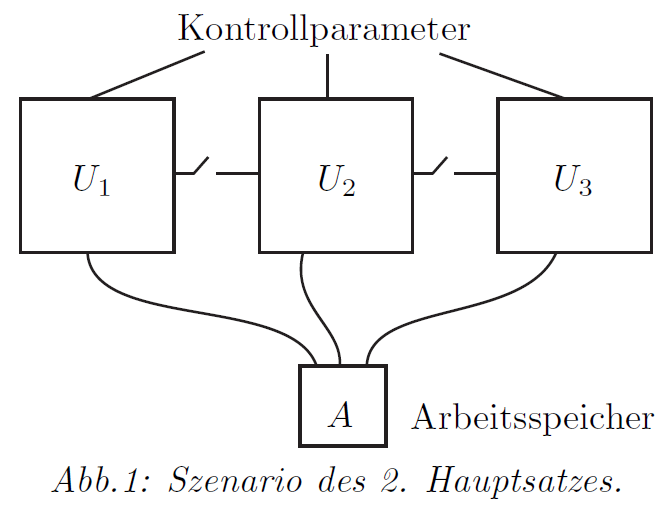
\includegraphics[width=0.5\textwidth,angle=0]{Bilder/Zweiter_HS.png}
%\captionof{figure}{}\medskip
\label{fig:Zweiter_HS}
\end{center}
Zum Aufbau: man hat ein Gesamtsystem aus mehreren einfachen Teilsystemen vorliegen, sowie einen Speicher für mechanische Arbeit. Zudem ist der Wärmekontakt zwischen den Teilsystemen quasi per Schalter regelbar. Bei sehr großen Teilsystemen ist zu beachten, dass diese ihren Zustand bei Kontakt mit kleinen Systemen kaum ändern werden (immer noch viel innere Energie/ Wärme da), solche Teilsysteme nennt man Wärmebäder.

	\anm{der Arbeitsspeicher ist natürlich aufgrund der Energieerhaltung nicht ohne eine Zustandsänderung (z.B. Wärmeabgabe) in einem Teilsystem aufladbar. Eine solche selbstversorgende Maschine, die nach einmaliger Energiezufuhr von außen ewig autark weiterlaufen würde, nennt man Perpetuum Mobile 1. Art. Sie ist nach dem 1. Hauptsatz nicht möglich/ verboten.}

Der 2. Hauptsatz der Thermodynamik macht nun eine Aussage über das Verhalten des Gesamtsystems und seiner Eigenschaften bei Zustandsänderungen (verursacht durch Änderung der Kontrollparameter oder Wärmeaustausch danach). Man kann ihn auf verschiedene Weisen formulieren:

\begin{itemize}
\item[(i)] Der Wärmefluss bei einer Zustandsänderung hat eine Vorzugsrichtung, sie fließt immer vom wärmeren zum kälteren Körper.

\item[(ii)] Eine Aufladung des Arbeitsspeichers auf Kosten der inneren Energie eines Teilsystems ist nicht möglich, es müssen sich alle ändern. Ein solches Perpetuum Mobile 2. Art ist nicht möglich (oft in Widerspruchsbeweisen benutzt).

\item[(iii)] Nach Max Planck und William Kelvin: $"$Es ist unmöglich, eine periodisch arbeitende Maschine zu konstruieren, die nichts weiter bewirkt, als Hebung einer Last und Abkühlung eines Wärmereservoirs.$"$ Das Problem ist nämlich, dass man immer noch andere beteiligte Teilsysteme hat, die dann auch am Wärmeaustausch beteiligt werden.
\end{itemize}


Rein mathematisch erhält man im Szenario eines einzelnen Systems bei adiabatischer Zustandsänderung, dass $U_{Anfang} = U_{Ende}$ gelten muss (Kreisprozess; kein Arbeitsgewinn aus der inneren Energie, siehe oben), woraus folgt, dass die Kurven mit gleichem Startpunkt und $\delta Q = 0$ (Bedingung für adiabatisch) eine Teilfläche von $\mathcal{Z}$ bilden, die man Adiabatenfläche nennt (alle Punkte auf dieser Fläche sind mit adiabatischen Prozessen erreichbar). Jede zu diesem Prozess senkrechte Funktion $\tilde{S}: \mathcal{Z} \rightarrow \mathbb{R}$ (deren Gradient diesen Prozess als Nullkurve hat, durch deren Konstanzflächen der Prozess also läuft, siehe bei \eqref{eq:nullkurve}) nennt man jeweils empirische Entropie.

	\anm{man erhält so die isentropen Zustandsänderungen ($dS = 0$)\\
$\Rightarrow$ alle Zustände auf einer Adiabatenfläche haben die gleiche Entropie (sind isentrop)}

Eine weitere Formulierung des 2. Hauptsatzes lautet in diesem Zusammenhang:
\begin{itemize}
\item[(iv)] Die Entropie eines Systems kann bei einem Prozess nur zunehmen ($dS > 0$). ! sogar $\geq \frac{\delta Q}{T}$ !
\end{itemize}\bigskip

Beispiel (Bestimmung der Adiabatenflächen eines idealen Gases):\\
Die Zustandsgleichung ist hier $U = \frac{f}{2}\, pV$ und das Arbeitsdifferential $\delta A = p\, dV$.
\begin{equation}
0 = dU + \delta A = \frac{f}{2} \qty(p\, dV + V\, dp) +p\, dV = \qty(\frac{f}{2} + 1) p\, dV + \frac{f}{2} V\, dp
\end{equation}
Nach Einführen des Adiabatenexponents $\kappa = \frac{f/2 + 1}{f/2} = \frac{f + 2}{f} = 1 + \frac{2}{f}$ wird das zu
\begin{equation}
0 = \kappa \frac{dV}{V} + \frac{dp}{p} = d\qty(\kappa \ln(V) + \ln(p)) = d\qty(\kappa \ln(pV)) = d\qty(\ln(pV^\kappa))
\end{equation}
die Adiabatenflächen erfüllen also $pV^\kappa = const.$  (steiler als Isotherme $pV = const.$).

%verschwindet das Wegintegral über $dU$ und da bei einem adiabatischen Prozess gerade $dU = \delta A$ gilt, verschwindet auch das Wegintegral über $\delta A$ (wegunabhängig !!).


	\subsection{Carnot-Prozesse}
Ein Carnot-Prozess (letztendlich Gedankenexperiment) ist ein Kreisprozess (ein System startet im gleichen Zustand wie es endet,die Kurve zum zugehörigen Prozess ist also geschlossen), aufgeteilt in vier Phasen (abwechselnd isotherm, adiabatisch). Untersucht wird dabei ein einfaches System $E$ im Zustand $(\tilde{T}_+, \tilde{S}_+)$ in Kontakt mit zwei Wärmebädern der empirischen Temperaturen $\tilde{T}_+$, $\tilde{T}_-$.\\
Bei jedem Prozess $\mathcal{C}_i$ wird vom System $E$ Wärme $Q_i \equiv \delta Q$ aufgenommen/ abgegeben und Arbeit $A_i \equiv \delta A$ verrichtet (VZ jeweils abhängig von Richtung des Prozesses).

\begin{center}
%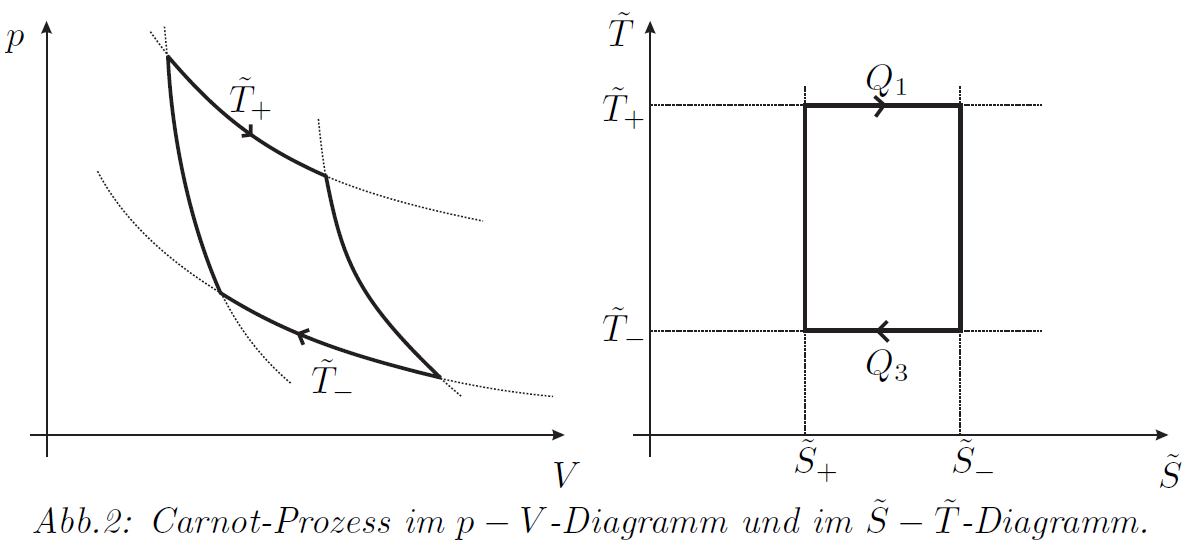
\includegraphics[width=0.8\textwidth,angle=0]{Bilder/Carnot.png}
%\captionof{figure}{}\medskip
\label{fig:Carnot}
\end{center}

Zur Erklärung: haben zwei isotherme Prozesse $\mathcal{C}_1$, $\mathcal{C}_3$ mit Wärmeänderung $Q_1$,  $Q_3$ (laufen bei gleichem $T = \tilde{T}_+/\, \tilde{T}_-$ ab $\rightarrow$ Wichtig: $\Delta Q \nRightarrow \Delta T$ !) %; hier wird keine Arbeit vom System verrichtet, $A_1 = 0 = A_3$) 
und zwei adiabatische $\mathcal{C}_2$, $\mathcal{C}_4$ mit $Q_2 = 0 = Q_4$ (war ja gerade Bedingung; dort bleibt Entropie konstant).\\
%; hier verrichtet das System eine Arbeit $A_2$, $A_4$).
Die vom System verrichtete Arbeit wird hier nicht näher beleuchtet, da es gar nicht explizit benötigt wird, es reicht hier der Zusammenhang $A_{Ges} = \sum \limits_i A_i$.

Bei Kontakt mit dem Wärmebad $\tilde{T}_+$ nimmt das betrachtete einfache System $E$ also die Wärme $Q_1 > 0$ auf, bei Kontakt mit $\tilde{T}_-$ gibt es $Q_3 < 0$ ab (können nicht das gleiche VZ haben, da sonst dauerhafter Energiegewinn auf Kosten des Wärmebades, was vom 2. Hauptsatz verboten wird). Da jedoch im Allgemeinen $\abs{Q_1} \neq \abs{Q_3}$ ist, hat man nach diesem Prozess eine andere Energie im System $E$ (und dementsprechend auch in den beiden Wärmebädern), als davor.

Je nachdem, in welche Richtung der Prozess abläuft, hat man so eine Wärmekraftmaschine (Arbeit aus Wärme, also Umwandlung von thermischer Energie in mechanische $\Rightarrow Q_1 + Q_3 > 0$) oder eine Wärmepumpe (Temperaturunterschied $\Delta T$, also Wärme, aus Arbeit $\Rightarrow Q_1 + Q_3 < 0$) konstruiert.\\
Das Besondere am Carnot-Prozess ist dabei die Reversibilität: wenn man also nach dem Kontakt der Reihenfolge $\tilde{T}_+ \rightarrow \tilde{T}_-$ den umgekehrten Prozess $\tilde{T}_- \rightarrow \tilde{T}_+$ ausführt, so sind alle beteiligten Teilsysteme danach wieder im Ausgangszustand (bei $\pm 0$).

Mathematisch kann man bei einem Kreisprozess $\mathcal{C}_{Ges} = \mathcal{C}_1 + \mathcal{C}_2 + \mathcal{C}_3 + \mathcal{C}_4$ schreiben:
\begin{equation}
0 = \oint_{\mathcal{C}_{Ges}} dU = \oint_{\mathcal{C}_{Ges}} \qty(Q_{Ges} - A_{Ges}) = \sum \limits_i Q_i - \sum \limits_i A_i \; \Leftrightarrow \; Q_1 + Q_3 = A_{Ges}
\end{equation}
	\anm{wir dürfen das Integral so einfach im $(\tilde{S}, \tilde{T})$-Raum bestimmen, da es bei Differentialformen ja unabhängig von der Parametrisierung ist !}

Satz: bei allen Carnot-Prozessen zwischen $\tilde{T}_+$ und $\tilde{T}_-$ ist das Verhältnis 
\begin{equation}\label{eq:carnot}
\frac{\abs{Q_{3}}}{Q_1} = const.\, .
\end{equation}
Der Carnot-Wirkungsgrad einer idealen Wärmekraftmaschine ist definiert als
\begin{equation} \eta_C = \frac{Q_1 + Q_3}{Q_1} = 1 - \frac{\abs{Q_{3}}}{Q_1} \equiv \frac{\text{abgegebene Arbeit } A_{Ges}}{\text{aufgenommener Wärme } Q_{Ges}} < 1,
\end{equation}
hier wird erfasst, welcher Anteil der aufgenommenen Wärmeenergie in nutzbare Arbeit/ Nutzarbeit umgewandelt werden kann (nicht vollständig möglich nach 2. Hauptsatz, da man sonst auf Kosten des Wärmebads $\tilde{T}_+$ Energie gewinnen würde).

Mit einer realen, periodisch arbeitenden Maschine (stellt auch Kreisprozess dar; das beste Beispiel ist die Dampfmaschine, die man als Wärmekraftmaschine auf dieser Basis konstruiert hat) können sogar nur Wirkungsgrade $\eta < \eta_C < 1$ erreicht werden (viele Verluste, da das System $E$ ja nicht wärmeisoliert ist, zusätzlich Reibung etc.).\\
Die Behandlung/ Idealisierung eines realen Prozesses als Carnot-Prozess wird oft zur Optimierung des Wirkungsgrades $\eta$ genutzt und auch Carnotisierung genannt.

%Kreisprozesse toll, da Anfang = Ende und dann Wegintegral = 0 ???


	\subsection{Absolute Temperatur und Entropie}
Nächster Schritt: Auswerten des 2. Hauptsatzes und Ausnutzen von Carnot-Prozessen

Bisher haben wir die Größen Temperatur und Entropie nur empirisch betrachtet, also relativ zueinander. Bei der Angabe von Experiment-übergreifenden, absoluten Werten für diese Größen hilft die Kombination von zwei Carnot-Prozessen (mit $Q'_3 = -Q_1$).\\
Man nehme dazu drei Wärmebäder der empirischen Temperaturen $\tilde{T}_- < T_0 < \tilde{T}_+$. $\mathcal{C}$ bezeichnet dabei den zwischen $\tilde{T}_-$, $T_0$ und $\mathcal{C}'$ den zwischen $T_0$, $\tilde{T}_+$.
\begin{center}
%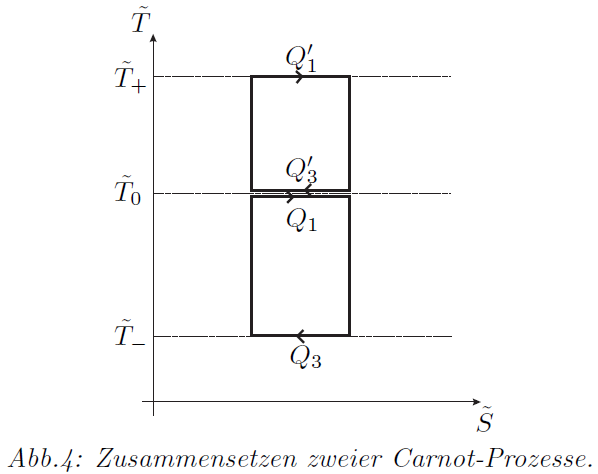
\includegraphics[width=0.5\textwidth,angle=0]{Bilder/Carnot_doppelt.png}
%\captionof{figure}{}\medskip
\label{fig:Carnot_doppelt}
\end{center}
Den zusammengesetzte Carnot-Prozess $\mathcal{C}''$ zwischen $\tilde{T}_-$,$\tilde{T}_+$ bildet dabei das äußere Rechteck (ohne Durchlaufen $Q_1$, $Q'_3$).

Nach Satz \eqref{eq:carnot} können wir unabhängig von der expliziten Form des Prozesses $\mathcal{C}''$ $f(\tilde{T}_+, \tilde{T}_-) = \frac{\abs{Q''_3}}{Q''_1}$ (wohldefiniert !) setzen. In der Abbildung \ref{fig:Carnot_doppelt} ist gut erkennbar, dass $Q''_1 = Q'_1$ und $Q''_3 = Q_3$, weshalb wir schreiben können (da offensichtlich $Q'_3 = -Q_1$):
\begin{equation}
f(\tilde{T}_+, \tilde{T}_-) = \frac{\abs{Q''_3}}{Q''_1} = \frac{\abs{Q_3}}{Q'_1} = \frac{\abs{Q_3}}{Q_1} \frac{\abs{Q'_3}}{Q'_1} = f(\tilde{T}_0, \tilde{T}_-) f(\tilde{T}_+, \tilde{T}_0)
\end{equation}

Setzt man nun $\tilde{T}_0$ auf einen beliebigen, aber festen Wert, ändert die Variable $\tilde{T}_+$ zu $\tilde{T}$ und setzt $\tilde{T}_-$ ebenfalls auf einen konstanten Wert, so ist $f(\tilde{T}_0, \tilde{T}_-) := T_0 = const.$ und wir können $f(\tilde{T}_+, \tilde{T}_-)$ als Temperaturskala verwenden:
\begin{equation}
T(\tilde{T}) = f(\tilde{T}_0, \tilde{T}) \cdot T_0 .
\end{equation}
Die Funktion $T$ ist nun die absolute Temperatur, die von nun an immer statt der empirischen verwendet wird. $T$ ist natürlich nicht eindeutig, da $T_0$ (dimensionsbehaftet, z.B. $°\celsius$, $°\kelvin$) beliebig ist, bekannte Beispielwerte sind hier $T_0 \equiv$ Tripelpunkt von Wasser bei der Celsius-Skala oder $T_0 = 273,15$ bei der Kelvin-Skala (messen Werte von $T$ dann relativ zu/ in Einheiten von $T_0$, also eigentlich in der Form: dieses $\Delta T$ ist doppelt so groß wie $T_0$).

	\anm{wegen $\frac{\abs{Q_3}}{Q_1} = \frac{T(\tilde{T}_-)}{T(\tilde{T}_+)} := \frac{T_-}{T_+}$ kann man auch schreiben: $\eta = 1 - \frac{T_-}{T_+} = \frac{T_+ - T_-}{T_+}$.}


Analog können wir nun auch die empirische Entropie $S$ ersetzen, was wichtig wird, da $S$ ja mit den interessanten Adiabatenflächen zusammenhängt.\\
Wir fixieren also den beliebigen, festen Wert $S_0$ einer ebenfalls beliebigen, aber festen Adiabatenfläche (dient als Referenz). Dann ist die Entropie einer anderen Adiabatenfläche, die über einen isothermen Prozess von der Referenzfläche zu erreichen ist (Flächen also über eine Kurve $\mathcal{C}$ verbunden mit $T = const.$ auf $\mathcal{C}$), gerade
\begin{equation}\label{eq:entropy}
S = S_0 + \frac{1}{T} \int_\mathcal{C} \delta Q .
\end{equation}
$S$ ist die (absolute) Entropie (wegunabhängige Definition, deshalb wohldefiniert). Tatsächlich ist die Analogie Entropie als Maß von Ordnung ist oft auch irreführend, aber in dem Sinne gerechtfertigt, dass es leichter ist, eine heile Tasse kaputt zu machen also eine kaputte Tasse wieder zusammen zu setzen.

Wir hatten ja bereits, dass $dS$ und $\delta Q$ beide auf den Adiabatenflächen verschwinden, also die gleichen Konstanzflächen haben. Damit können wir ein $\lambda$ (integrierender Faktor) finden, sodass $dS = \lambda \, \delta Q$. Zu beachten ist, dass das $\lambda$ entlang eines nicht-adiabatischen Weges bestimmt werden muss, sonst gilt die Gleichheit $\forall \lambda$, weil dort ja gerade $\delta Q = 0 = dS$. Geeignet ist z.B. ein isothermer Weg wie in \eqref{eq:entropy}. Das ergibt
\begin{equation}
\lambda = \frac{1}{T} \; \Leftrightarrow \; dS = \frac{\delta Q}{T}
\end{equation}

Wir können die Entropie also insbesondere als Aufsammeln/ Abgeben von Wärme $\delta Q$ bei Durchlaufen eines Prozesses $\mathcal{C}$ normiert mit $T$ betrachten. Daraus folgt direkt, dass bei adiabatischen Prozessen ($\delta Q = 0$) $dS = 0 \; \Leftrightarrow \; S = const.$ gilt, die Entropie bleibt also erhalten. Dies gilt weiterhin bei zusammengesetzten Systemen, da dort $dS_{Ges} = \frac{\delta Q_{Ges}}{T} = \sum\limits_i \frac{\delta Q_i}{T} = \sum\limits_i dS_i$ (folgt also, da andere Größen wie $\delta Q$ auch additiv). Insbesondere folgt daraus, dass bei Carnot-Prozessen die Entropie $S_{Ges}$ erhalten bleibt ($dS_{Ges} = 0$, Herleitung in OneNote zu HÜ 2 Aufgabe 1).

Betrachtet man nun jedoch zwei einfache Systeme $-$ und $+$ mit Temperaturen $T_- < T_+$ und bringt diese in Wärmekontakt, so kommt es aufgrund des 2. Hauptsatzes zu einem Wärmefluss von $+$ zu $-$, der zum Herstellen eines Gleichgewichtszustandes nötig ist. Während dieses Ausgleich-Prozesses kommt es also zu Energie-/ Wärmeänderungen $\delta Q_- > 0$ (Aufnahme), $\delta Q_+ < 0$ (Abgabe), wobei $\delta Q_- = \delta Q_+$ gelten muss (1. Hauptsatz/ Energieerhaltung). Für die Entropieänderung erhält man dann gerade
\begin{equation}
dS = dS^{(-)} + dS^{(+)} = \frac{\delta Q_-}{T_-} + \frac{\delta Q_+}{T_+} = \delta Q_- \qty(\frac{1}{T_-} - \frac{1}{T_+}) > 0 .
\end{equation}
Hier ist die Entropie des Gesamtsystems also nicht erhalten, sie nimmt zu (allgemeingültige Aussage für abgeschlossene Systeme) ! Durch Zuschalten eines speziellen Wärmebades ließe sich zwar auch jede andere Zustandsänderung (also jeder andere Wert von $dS$) erreichen, aber nur im dann nicht mehr abgeschlossenen System aus $-$ und $+$ (im Gesamtsystem aus $-$, $+$ und Wärmebad hätte man wieder $dS > 0$ !).\\
Dies ist die Bestätigung der Formulierung (iv) des 2. Hauptsatzes.

Sehr interessant ist, dass solche Austauschprozesse mit $dS > 0$ nicht rückgängig zu machen sind (zumindest nicht im betrachteten abgeschlossenen System), adiabatische Prozesse mit $dS = 0$ aber schon (Umkehrung der Richtung durch Umkehrung der Wärmekontakte und Kontrollparameter).\\
Das ist kein Zufall/ Spezialfall, die Entropie bildet allgemein ein Maß für die Erreichbarkeit eines Zustands und somit die Machbarkeit einer Zustandsänderung (bzw. auch für die Machbarkeit der Umkehrung dieser Änderung):
\begin{itemize}
\item[-] Prozesse mit $dS = 0$ heißen reversibel und sind durch einen adiabatischen Prozess erreichbar (auch Umkehrung möglich)
\item[-] Prozesse mit $dS > 0$ heißen irreversibel (nicht umkehrbar); bei größeren Werten von $dS$ ist die Änderung also schwieriger $\rightarrow$ logisch, da dann große Wärmemenge $\delta Q$ bei evtl. kleiner Temperatur $T$ aufgewendet werden muss
\end{itemize}\bigskip

Beispiel (Bestimmung der Entropie eines idealen Gases):\\
Allgemein gilt beim idealen Gas $\delta A = p\, dV$ (siehe oben). Weiter ist auf einer Isothermen nach dem Gesetz von Boyle-Mariotte  $pV \sim T = const. \Leftrightarrow pV := \theta = const.$, es gilt also $U = \frac{f}{2}\, pV = \frac{f}{2}\, \theta = const.$. Mit dem ersten Hauptsatz folgt dann
\begin{equation}
dS = \frac{\delta Q}{T} = \frac{dU + \delta A}{T} = \frac{dU}{T} + \frac{p\, dV}{T}
\end{equation}

Im Koordinatensystem $(\theta, V)$ lautet dieser Ausdruck (mit $p = \frac{\theta}{V}$):
\begin{equation}
dS = \frac{d\qty(f/2\, \theta)}{T} + \frac{\theta/V\, dV}{T} = \frac{f}{2T}\, d\theta + \frac{\theta}{VT}\, dV
\end{equation}

Da $dS$ exakt ist, muss sie auch geschlossen sein und es folgt wegen der Symmetrie der gemischten zweiten Ableitungen und da $T = const.$:
\begin{equation}
\qty( \pdv{(\theta/TV)}{\theta})_V = \qty( \pdv{(f/2T)}{V})_\theta = 0
\end{equation}

Aus dem zweiten Gleichzeichen folgt, dass $\chi := \theta/T$ (extensive Größe; später: $\chi = N\cdot R$) unabhängig von $\theta$ sein muss ($V$ wird ja festgehalten; Gasthermometer also gut geeignet, gibt absolute Temperatur). Einsetzen von $\theta = \chi T$ ergibt den endgültigen Ausdruck
\begin{equation}
dS = \chi \qty( \frac{f}{2}\, \frac{dT}{T} + \frac{dV}{V}) \; \Leftrightarrow \; S(T,V) = S_0 + \chi \qty( \frac{f}{2} \ln\qty( \frac{T}{T_0}) + \ln\qty( \frac{V}{V_0}) )
\end{equation}

In anderen Koordinatensystemen würde man folgende Ausdrücke erhalten:
\begin{align}
S(p,V) = S_0 + \chi \qty( \frac{f}{2} \ln\qty( \frac{p}{p_0}) + 2\ln\qty( \frac{V}{V_0}) )
\\
S(U,V) = S_0 + \chi \qty( \frac{f}{2} \ln\qty( \frac{U}{U_0}) + \ln\qty( \frac{V}{V_0}) )
\end{align}
Dabei wurde Proportionalitäten und Kürzen von Konstanten im Bruch genutzt.



	\subsection{Gleichgewichtsbedingungen}
Beispiel (zwei einfache Systeme $1$ und $2$ in Wärmekontakt):\\
Wie bereits festgehalten, wird sich im zusammengesetzten System ein Gleichgewicht einstellen (in dem $T^{(1)} = T^{(2)}$). Die Art des Gleichgewichts ist dabei abhängig vom Prozess, der eventuell dazwischen stattfindet:
\begin{itemize}
\item[1.] spontaner Energieausgleich: hier bleibt die Gesamtenergie $U = U^{(1)} + U^{(2)}$ des Systems erhalten, die Entropie $S = S^{(1)} + S^{(2)}$ aber wächst ($\Rightarrow dU = 0, \, dS > 0$)\\ %  \Leftrightarrow dU^{(1)} = -dU^{(2)} ??? -> bei S eben nicht
$\rightarrow$  Einstellen von maximaler Entropie bei fester innerer Energie

\item[2.] Verrichtung von Arbeit durch reversibel arbeitende Wärmekraftmaschinen: hier bleibt $U = U^{(1)} + U^{(2)} - \delta A$ aufgrund des Verlustes an mechanische Arbeit $\delta A$ nicht erhalten, die Entropie $S = S^{(1)} + S^{(2)}$ hingegen schon ($\Rightarrow dU < 0, \, dS = 0 $)\\ %  \Leftrightarrow dS^{(1)} = -dS^{(2)} ??? -> bei U eben nicht (dann wäre T1=T2, allerdings nicht = lambda)
$\rightarrow$ Einstellen von minimaler Energie bei fester Entropie

\item[$\Rightarrow$] beide liefern aber ein äquivalentes Ergebnis, wie man schnell mithilfe von Lagrange-Multiplikatoren (keine Konstanten, sondern Funktionen !) sieht: mit der jeweiligen Bedingung $d(U - \lambda S) = 0$ ($U$ extremal bei festem $S$ und festen Kontrollparametern) bzw. $d(S - \lambda' U) = 0$ ($S$ extremal bei festem $U$ und festen Kontrollparametern) folgt
(beide Bedingungen sind äquivalent mit $\lambda' = 1/\lambda$)
\begin{align}
dU^{(i)} &= \delta Q^{(i)} - \delta A^{(i)} = T^{(i)} dS^{(i)} - \delta A^{(i)} = T^{(i)} dS^{(i)} \; (\text{Fall 1})
\notag\\
\Rightarrow dU - \lambda dS &= dU^{(1)} + dU^{(2)} - \lambda dS^{(1)} + dS^{(2)}
\notag\\
&= \qty(T^{(1)} - \lambda)\, dS^{(1)} + \qty(T^{(2)} - \lambda)\, dS^{(2)}
\notag\\
\Leftrightarrow T^{(1)} = \lambda &= T^{(2)} \; (\text{da } dS^{(1)} \neq dS^{(2)})
\end{align}
\end{itemize}

Beispiel (Doppelkolben):\\
\begin{center}
%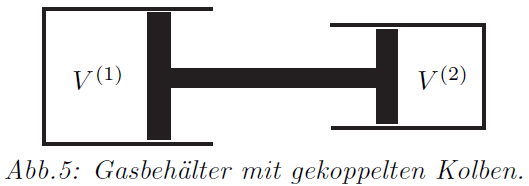
\includegraphics[width=0.5\textwidth,angle=0]{Bilder/Kolben.png}
%\captionof{figure}{}\medskip
%\label{fig:Carnot_doppelt}
\end{center}
Wir erweitern nun die Anzahl der Nebenbedingungen, indem wir Änderungen der Kontrollparameter (hier die Volumina $V^{(1)}, \, V^{(2)}$ eines Gases) zulassen. Sind die beiden Kolben mit einer Stange verbunden, so ergibt sich die NB zu
\begin{equation}\label{eq:NBkolben}
\frac{V^{(1)}}{a_1} + \frac{V^{(2)}}{a_2} = const. .
\end{equation}
Bei Auslenkung der Kolben (System in Nicht-Gleichgewichtszustand), so werden die Kolben eine Schwingung ausführen, bis die Schwingungsenergie durch irreversible Prozesse (z.B. Reibung $\equiv$ Wärmeentwicklung) aufgebraucht ist (dann Gleichgewicht erreicht). Dabei wächst die Entropie nach dem 2. Hauptsatz an und erreicht ihr Maximum im Gleichgewichtszustand.\\
Eine Alternative, die nun näher beleuchtet werden soll, ist das Verschieben von Energie in einen Arbeitsspeicher (gerade so viel, dass es zu keiner Schwingung kommt). Wir wollen also $dU = 0$ unter Berücksichtigung von \eqref{eq:NBkolben}, $S^{(1)} = const.$, $S^{(1)} = const.$ (getrennte Betrachtung von $S$, da Systeme wärmeisoliert sein sollen). Da zusätzlich eventuell zum Ausgleichen anderer Kräfte eine Arbeit $\delta A^{(i)} = p^{(i)} dV^{(i)}$ wird, erhält man mit den drei nötigen Lagrange-Multiplikatoren $\lambda_j$ zu den drei NB:
\begin{align}
dU^{(i)} &= T^{(i)} dS^{(i)} - p^{(i)} dV^{(i)} 
\notag\\
\Rightarrow 0 &= dU - \lambda_1 dS^{(1)} - \lambda_2 dS^{(2)} - \lambda_3 \qty(\frac{V^{(1)}}{a_1} + \frac{V^{(2)}}{a_2}) 
\notag\\
&= \qty( T^{(1)} -\lambda_1)\, dS^{(1)} + \qty(T^{(2)} - \lambda_2)\, dS^{(2)} - \qty(p^{(1)} + \frac{\lambda_3}{a_1})\, dV^{(1)} - \qty(p^{(2)} + \frac{\lambda_3}{a_2})\, dV^{(2)}
\notag\\
&= - \qty(p^{(1)} + \frac{\lambda_3}{a_1})\, dV^{(1)} - \qty(p^{(2)} + \frac{\lambda_3}{a_2})\, dV^{(2)}
\notag\\
\Leftrightarrow & - \qty(a_1 \, p^{(1)} + \lambda_3)\, \frac{dV^{(1)}}{a_1} = \qty(a_2 \, p^{(2)} + \lambda_3)\, \frac{dV^{(2)}}{a_2}
\notag\\
\Leftrightarrow & - \qty(a_1 \, p^{(1)} + \lambda_3)\, d\qty(\frac{V^{(1)}}{a_1}) = \qty(a_2 \, p^{(2)} + \lambda_3)\, d\qty(\frac{V^{(2)}}{a_2})\label{eq:dglkolben}
\end{align}
Ableiten von \eqref{eq:NBkolben} ergibt die Bedingung
$$ -d\qty(\frac{V^{(1)}}{a_1}) = d\qty(\frac{V^{(2)}}{a_2})$$

und setzt man das in \eqref{eq:dglkolben} ein, erhält man
\begin{align}
\qty(a_1 \, p^{(1)} + \lambda_3)\, d\qty(\frac{V^{(2)}}{a_2}) &= \qty(a_2 \, p^{(2)} + \lambda_3)\, d\qty(\frac{V^{(2)}}{a_2})
\notag\\
\Leftrightarrow a_1 \, p^{(1)} &= a_2 \, p^{(2)}\label{eq:ergkolben}
\end{align}
Speziell, wenn lediglich das Gesamtvolumen $V = V^{(1)} + V^{(2)}$ erhalten werden soll (also $a_1 = 1 = a_2$), ist die Gleichgewichtsbedingung statt \eqref{eq:ergkolben} einfach $p^{(1)} = p^{(2)}$.

Beispiel (einfaches, evtl. zusammengesetztes System in Kontakt mit Wärmebad $B$):\\
Allgemeiner betrachten wir hier beliebige Kontrollparameter $\alpha_i$ mit den zugehörigen Nebenbedingungen und suchen das Minimum von $U + U_B$ bei festem $S + S_B$.
\begin{equation}
\Rightarrow d\qty( U + U_B) = 0 = d\qty( S + S_B) \; \Leftrightarrow \; dU = -dU_B, \, dS = - dS_B
\end{equation}

Bei festem $\alpha$ (als Satz der Kontrollparameter) variiert also nur die Aufteilung der Entropie zwischen $S$ und $S_B$. Mit dem zustandsunabhängigen Faktor $T_B$ gilt dann
\begin{equation}
dU_B = T_B dS_B = -T_B dS = -dU
\end{equation}
Betrachten wir $T_B$ als Lagrange-Multiplikator, so ist es also die Aufgabe, das Minimum von $U - T_B \, S$ zu finden. Wir definieren dann die Helmholtz'sche Freie Energie als
\begin{equation}\label{eq:freieen}
F \qty(T_B, \alpha) = \min\qty{U - T_B \, S: \alpha \text{ fest}} = \min\qty{U - T \, S: \alpha \text{ fest}}
\end{equation}
$F$ ist die Legendre-Transformierte der inneren Energie bezüglich $S$ (da $-\min{} = \max{}$) und steht für die Energie des Systems im Gleichgewichtszustand (dieser ist bei festem $T$, $V$ gerade darüber definiert, dass $F$ dort minimal sein muss).
Im Koordinatensystem $(S, \alpha)$ muss man dann nur noch das zugehörige $S$ finden, in dem das Gleichgewicht erreicht wird. Im Gleichgewichtszustand gilt natürlich auch $T_B = T$, sodass die Notation in \eqref{eq:freieen} gerechtfertigt ist.\\
Man hat nun die Variablen des Problems reduziert auf $T_B$ bzw. $T$ und man kann zur Lösung des Problems einfach $F \qty(T, \alpha)$ zu den gegebenen NB $\alpha$ berechnen.

	\anm{sehr ähnliches Vorgehen bei Volumentausch mit $B$ (dabei $p \equiv T$)}



	\subsection{Konvexität extensiver Zustandsgrößen}
Die Definition extensiver Zustandsgrößen war ja, dass bei einer Vervielfachung des Systems um einen Faktor $\lambda$ die Größe ebenfalls um $\lambda$ wächst. Beispiele sind die innere Energie $U$, die Entropie $S$, das Volumen $V$ oder die verschiedenen Stoffmengen $N_i$ der im System enthaltenen Stoffe, zusammengefasst in einem Vektor $\vec{N}$. Man kann nun aufgrund der eben beschriebenen Extensivität schreiben:
\begin{equation}\label{eq:lu}
U (\lambda S, \lambda V, \lambda \vec{N}) = \lambda U (S, V, \vec{N})
\end{equation}
Man nennt $U$ dann homogen vom Grad 1. Durch partielles Ableiten beider Seiten in \eqref{eq:lu} nach $\lambda$ an der Stelle $\lambda = 1$ erhält man das Euler-Theorem \eqref{eq:gdalmost} und daraus die Gibbs'sche Fundamentalrelation \eqref{eq:dUcoeff}
\begin{align}
\qty(\pdv{U}{S}) S + \qty(\pdv{U}{V}) V + \sum\limits_i \qty(\pdv{U}{N_i}) N_i &= U\label{eq:gdalmost}
\\
\Rightarrow dU = \qty(\pdv{U}{S}) dS + \qty(\pdv{U}{V}) dV + \sum\limits_i \qty(\pdv{U}{N_i}) dN_i &= T\, dS - p\, dV + \sum\limits_i \mu_i dN_i,\label{eq:dUcoeff}
\end{align}
wobei man die Größen $\mu_i$ als chemische Potentiale des jeweiligen Stoffes bezeichnet.\\
Da $S, V, \vec{N}$ eine Basis von $\mathcal{Z}$, also ein KS bilden, und die Darstellung \eqref{eq:dUcoeff} von $dU$ in einer Basis eindeutig ist, sind die Größen $T, p, \mu_i$ eindeutig und \eqref{eq:gdalmost} wird zur Euler-Gleichung der inneren Energie
\begin{equation}
U (S, V, \vec{N}) = T\, S - p\, V + \sum\limits_i \mu_i N_i .
\end{equation}

Auf ganz analogem Wege ($S$ auch homogen) erhält man die Sackur-Tetrode-Gleichung
\begin{equation}\label{eq:sacktetr}
S (U, V, N) = RN \qty(\frac{f}{2} \ln\qty(\frac{U}{U_0}) + \ln\qty(\frac{V}{V_0}) - \frac{f+2}{2} \ln\qty(\frac{N}{N_0}) + \frac{S_0}{RN_0}) .
\end{equation}

	\anm{die $x_0$-Terme sind nur Konstanten, die den $\ln$ dimensionslos machen $\rightarrow$ können so Gleichungen schön vereinfachen !}

$R = N_{Avogadro} \cdot k_B$ ist die allgemeine Gaskonstante, deren exakter Zahlenwert von den Einheiten von $T, N$ abhängt. Durch Differentiation nach $U$ erhält man die Ausdrücke
\begin{equation}
U = \frac{f}{2} RT, \; pV = RNT ???.
\end{equation}

Bringt man nun zwei Systeme der gleichen, homogenen Substanz in Wärmekontakt und wartet ab, bis es im Gleichgewicht (bei minimalem $U$) ist, so erhält man mit $U^1 = U^2 = U^{Ges}$ (Energiewerte zwar unterschiedlich, aber aus gleicher Funktion bestimmt wird; logisch, da Art des Zustands, nämlich homogen, bei allen gleich)

(Annahmen: nur adiabatische Prozesse $\Leftrightarrow S = const.$, eingeschränktes Volumen $\Leftrightarrow V^{Ges} = V^1 + V^2 = const.$, Teilchenzahlerhaltung $\Leftrightarrow \vec{N}^{Ges} = \vec{N}^1 + \vec{N}^2 = const.$)
\begin{equation}
U(S^{(1)} + S^{(2)}, V^{(1)} + V^{(2)}, \vec{N}^{(1)} + \vec{N}^{(2)}) \leq U(S^{(1)}, V^{(1)}, \vec{N}^{(1)}) + U(S^{(2)}, V^{(2)}, \vec{N}^{(2)}).
\end{equation}
Wiederum mit genau analogen Überlegungen zur maximalen Entropie erhält man
\begin{equation}
S(U^{(1)} + U^{(2)}, V^{(1)} + V^{(2)}, \vec{N}^{(1)} + \vec{N}^{(2)}) \geq S(U^{(1)}, V^{(1)}, \vec{N}^{(1)}) + S(U^{(2)}, V^{(2)}, \vec{N}^{(2)}).
\end{equation}
Man nennt $U (S, V, \vec{N})$ subadditiv (bei Zusammensetzen kann man nur Energie durch Arbeit o.Ä. verlieren, aber keine gewinnen) und $S (U, V, \vec{N})$ superadditiv (kann bei einem Prozess nach dem 2. Hauptsatz ja nur zunehmen, außer bei Carnot).

Kombiniert man diese Additivitätseigenschaften mit der Homogenität vom Grad 1, so erhält man die Konvexität von $U (S, V, \vec{N})$ und Konkavität von $S (U, V, \vec{N})$
\begin{align}
U(\lambda S^{(1)} + (1-\lambda)\, S^{(2)}, \lambda V^{(1)} + (1-\lambda)\, V^{(2)}, \lambda \vec{N}^{(1)} + (1-\lambda)\, \vec{N}^{(2)})
\notag\\
\leq \lambda U(S^{(1)}, V^{(1)}, \vec{N}^{(1)}) + (1-\lambda)\, U(S^{(2)}, V^{(2)}, \vec{N}^{(2)})
\\
S(\lambda U^{(1)} + (1-\lambda)\, U^{(2)}, \lambda V^{(1)} + (1-\lambda)\, V^{(2)}, \lambda \vec{N}^{(1)} + (1-\lambda)\, \vec{N}^{(2)})
\notag\\
\geq \lambda S(U^{(1)}, V^{(1)}, \vec{N}^{(1)}) + (1-\lambda)\, S(U^{(2)}, V^{(2)}, \vec{N}^{(2)}).
\end{align}

Dies kann man als Stabilitätsbedingung betrachten, da es impliziert, dass man aus dem inhomogenen Zustand eines Materials Energie gewinnt, wenn man es homogen macht (da $U$ minimal bei homogen muss inhomogener höhere Energie haben).



	\subsection{*Konvexe Funktionen und Legendre-Transformationen*}
Der Wert der zweiten Ableitung $f'' \geq 0$ ist hinreichend für konvex (wenn $f$ dfb.; allgemeiner soll die Hesse-Matrix $D^2 f$ positiv definit sein), aber nicht notwendig.

Doppelte Anwendung Legendre gibt konvexe Hülle der Funktion (gleich der Funktion wenn konvex) -> Involutivität

	\anm{konkav ist als Definition nicht sinnvoll, da man es als Gegensatz von konvexer Menge definieren kann, aber dann könnte man auch einfach nicht konvex sagen. Linsen heißen konvex oder konkav, da man dort eine Krümmung von der optischen Achse aus hat (hier also sinnvoll).}

Supergraph ist abgeschlossen genau dann wenn f unterhalbstetig ist (Gesundheit; sind Legendre-Transformierte immer) -> heißt, dass man bei Unstetigkeitsstelle immer unteren Funktionswert nimmt

Legendre-Trafo ändert zwar auch die transformierte Größe, aber insbesondere den Variablensatz der Funktion -> dabei bleiben aber die Informationen über das System erhalten, da ja eine doppelte Legendre wieder die Funktion gibt (enthält ja selbe Infos dann), sie kann also nicht verloren gehen

Beispiel: Legendre von $U(S, V; N)$ bezüglich $(S, V)$ auf die neuen Variablen $(T, p)$ ist das (negative) Gibbs'sche Potential $G(T, p, N) = -\qty(\mathcal{L}U(\cdot, \cdot, N)) (T, p, N)$



	\subsection{Thermodynamische Potentiale}
Thermodynamische Potentiale (auch Fundamentalgleichungen genannt) sind Funktionen, die bereits alle Informationen über ein System enthalten. Diese Information steckt aber in den funktionalen Abhängigkeiten, es kommt also vor allem darauf und weniger auf die genaue Größe/ Funktion an. Man betrachtet dazu oft die Differentiale dieser Größe, da man so die jeweiligen Koeffizienten erhält (eben z.B. $p = -\qty(\pdv{U}{V})_T$). Relevant werden sie vor allem auch als Andockpunkt an die Statistische Mechanik, wo sie die sogenannte Mikrokanonische Gesamtheit beschreiben.

Welches Potential man genau für ein gewisses System betrachtet, hängt dabei von den Kontrollmöglichkeiten ab, die einem zur Verfügung stehen, da man einen Teil der Argumente ja als Kontrollparameter hat.

	\anm{zur Notation: $N$ (nicht mehr $\vec{N}$ genannt) umfasst weiter die Stoffmengen $N_i$, aber auch alle anderen Kontrollparameter $\alpha$. Daher steht $\mu N$ für $\vec{\mu} \cdot \vec{N} =  \sum\limits_i \mu_i N_i$.}

Wichtige Beispiele für thermodynamische Potentiale sind:
\begin{itemize}

\item[-] Innere Energie $U(S, V, N)$:
\begin{equation}\label{key}
dU = T \, dS - p \, dV + \mu \, dN
\end{equation}
Es folgen sofort Relationen $\delta Q = T \, dS$, $\delta A = p \, dV - \mu \, dN$ sowie für die Koeffizienten $T(S, V, N) = \qty(\pdv{U}{S})_{V, N}$, $p(S, V, N) = -\qty(\pdv{U}{V})_{S, N}$, $\mu(S, V, N) = -\qty(\pdv{U}{N})_{S, V}$ (das sind aber alles keine thermodynamischen Potentiale !).

Zudem erhalten wir aus der Konvexität von $U$ Ungleichungen
\begin{align}
\qty(\pdv[2]{U}{V})_{S, N} &= -\qty(\pdv{p}{V})_{S, N} \geq 0
\\
\qty(\pdv[2]{U}{S})_{V, N} &= \qty(\pdv{T}{S})_{S, V} \geq 0
\\
\qty(\pdv[2]{U}{N})_{S, V} &= \qty(\pdv{\mu}{N})_{S, V} \geq 0
\end{align}
Daraus folgt z.B., dass Adiabaten ($dS = 0$) im $p$-$V$-Diagramm fallen.

Aus der Vertauschbarkeit der zweiten Ableitung folgen die Maxwell-Relationen:
\begin{align}
\qty(\pdv{T}{V})_S = -\qty(\pdv{p}{S})_V \hspace{2cm} \qty(\pdv{T}{p})_S = \qty(\pdv{V}{S})_p,
\\
\qty(\pdv{V}{T})_p = -\qty(\pdv{S}{p})_T \hspace{2cm} \qty(\pdv{p}{T})_V = \qty(\pdv{S}{V})_T
\end{align}

%Mit $-\qty(\pdv{p}{V})_S$, als negative Steigung einer Adiabaten im $p-V-$Diagramm.

schlecht: können Entropie nicht wirklich messen, daher ersetzen ?



\item[-] Freie Energie $F(T, V, N)$ (auch Kanonische Gesamtheit; gut bei Wärmekontakt):
\begin{align}\label{key}
F(T, V, N) &= U - TS = - \qty(\mathcal{L} U(\cdot, V, N)) (T, V, N)
\\
dF &= -S \, dT - p \, dV + \mu \, dN
\end{align}
$F$ ist also eine Legendre-Transformierte von $U$, wobei der Variablenwechsel $S \mapsto T$ durchgeführt wird. Daraus folgt direkt die Konkavität in $T$ und die Konvexität in $(V, N)$ (da $U$ ja insgesamt konvex). Zudem muss auch $F$ alle Informationen über das System enthalten, da $\mathcal{L} F = U$ (wieder, da $U$ konvex).

Bei einem isothermen Prozess ($dT = 0$) erhält man dann $dF = -\delta A$ und dass dann $F$ konvex ist (einzige konkave Variable $T$ weg). Es gilt dann analog zu $U$
\begin{equation}\label{key}
\qty(\pdv[2]{F}{V})_{T, N} = -\qty(\pdv{p}{V})_{T, N}
\end{equation}
Auch die Isothermen fallen also im $p$-$V$-Diagramm.



\item[-] ? Enthalpie $H(S, p, N)$, $H = U + pV$ (auch iwie mit Legendre), dann $G = H - TS$ ?



\item[-] Freie Enthalpie $G(T, p, N)$/ Gibbs'sches Potential (gut bei  Volumentausch):
\begin{align}\label{key}
G &= U - TS + pV = \mu N = - \qty(\mathcal{L} U(\cdot, \cdot, N)) (T, p, N)
\\
dG &= -S \, dT + V \, dp + \mu \, dN
\end{align}
$G$ ist also eine Legendre-Transformierte von $U$, wobei der Variablenwechsel $(S, V) \mapsto (T, p)$ durchgeführt wird. Daraus folgt direkt die Konvexität in $N$ und die Konkavität in $(T, p)$.

Bei einem isothermen, isobaren Prozess ($dT = 0 = dp$) gilt fast analog zu $F$ für die Arbeit $\delta A_{Ges} = \delta A - p\, dV = -dG$ (da der Teil $p\, dV$ nicht nutzbar ist, das soll aber $G$ darstellen).



\item[-] Großkanonisches Potential $J(T, V, \mu)$ (auch großkanonische Gesamtheit):
\begin{align}\label{key}
J &= -pV = F - \mu N = U - TS - \mu N = -\qty(\mathcal{L}U(\cdot, V, \cdot)) (T, V, \mu)
\\
dJ &= -S \, dT -p \, dV - N \, d\mu
\end{align}
$J$ ist also eine Legendre-Transformierte von $U$, wobei der Variablenwechsel $(S, N) \mapsto (T, \mu)$ durchgeführt wird. Daraus folgt direkt die Konvexität in $V$ und die Konkavität in $(T, \mu)$.

Relevant wird das bei bei Quantengasen, Bose-Einstein-Kondensaten (hier nicht).

\end{itemize}

Durch Ausnutzen von bekannten Gleichungen (ideales Gas, Adiabaten, etc.) kann man dann weitere Variablenwechsel durchführen.

$\rightarrow$ Guggenheim-Quadrat für einfaches Merken Zusammenhang dieser Größen



	\subsection{Phasenübergänge}
Zunächst muss natürlich der Begriff des Phasenübergangs definiert werden. Sehr anschaulich/ geometrisch ist ein Phasenübergang 1. Ordnung ein $"$Knick$"$ in einem thermodynamischen Potential, wo eben jenes also nicht mehr stetig differenzierbar ist (bezogen auf erste Ableitung, dort $"$Sprung$"$). Analog definiert man einen Übergang n-ter Ordnung als $"$Sprung$"$ der n-ten Ableitung eines thermodynamischen Potentials.

Beispiel Van-der-Waals-Gas:\\
(auch Reales Gas genannt im Kontrast zu Idealem Gas, selbst wenn es noch nicht ganz realistisch ist, siehe steigende Isotherme/ negativer Druck)

$$R = k_B !!!$$

to be continued....



Hier gilt die Energie-Zustandsgleichung (Druckzustandsgleichung nach Ersetzen $U$)
\begin{equation}\label{key}
S(U, V, N) = N R \ln\qty(\frac{1}{V_0} (V - b N)) + \frac{f}{2} N R \ln\qty( \frac{N_0}{V_0} \frac{U V + a N^2}{N V})
\end{equation}
Dabei sind $b \equiv$ Binnenvolumen, $a \equiv$ Binnendruck im Prinzip Fitparameter. Es folgt
\begin{equation}\label{key}
dS = \frac{1}{T} \qty(dU + p \, dV) \Rightarrow T = \qty(\pdv{S}{U})^{-1}, \, \frac{P}{T} = \pdv{S}{V}
\end{equation}

Im Plot aus der Vorlesung (Dateiname: 2020.10.29. vdW-Gas) sind die man die Isothermen zu verschiedenen Werten von $p$ und $V$ dargestellt. Ab einem kritischen Punkt bei $T_C = 8/3$ (dimensionslos durch Wahl der Konstanten, ist bei jedem Modell dieser Art so machbar) erkennt man, dass bei $T < T_C$ die Isotherme nicht mehr fällt, sondern steigt (bei kleinen $T$ wird dabei sogar der Druck $p$ negativ bei kleinen $V$)!\\
Sonst (bei $T \geq T_C$) erhält man monoton fallende Isothermen (genau richtig), aber der Rest ist unphysikalisch (widerspricht Stabilitätsbedingung des 2. Hauptsatzes) !

Das van-der-Waals-Gas kann also nicht die Realität beschreiben. Maxwell hat das Modell jedoch gerettet, indem er einen Sprung der Isotherme (weiter im $p$-$V$-Diagramm) eingeführt hat (die Maxwell-Konstruktion), sodass es keinen Widerspruch mehr gibt. Dieser Sprung ist ein Phasenübergang, da sich auf einmal das Volumen bei konstantem Druck ändert (funktioniert unter Mithilfe der Schwerkraft). Man erhält dann eine Phasenkoexistenz, links von der Geraden ist der flüssige Zustand und rechts ein Gas.

\begin{center}
%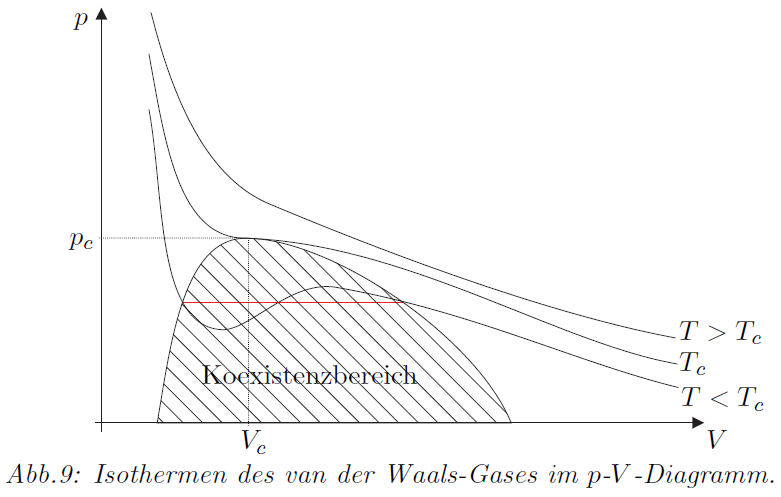
\includegraphics[width=0.6\textwidth,angle=0]{Bilder/maxwell.png}
%\captionof{figure}{}\medskip
\label{fig:}
\end{center}

Die Frage ist nun jedoch, wo man diesen Schnitt ansetzt, es scheint erst einmal willkürlich. Man macht es jedoch gerade so, dass die thermodynamischen Potentiale konvex in $V$ werden (man nimmt dabei genau die gleiche Fläche unter und über dem eigentlichen Graphen weg).\\
Man könnte auch sagen, dass aus einem $"$schlechten$"$ thermodynamischen Potential (unphysikalisch) ein $"$gutes$"$ gemacht wird (ist konvexe Hülle des $"$schlechten$"$).

Es tritt dabei auch ein Problem auf: wie z.B. in der Grafik erkennbar ist, liegen nun zwei Punkte mit gleichem Paar $(T, p)$ vor, es kommt also auch zu Knicken in der Freien Enthalpie $G$ und ein Zustand ist nicht wie normal eindeutig durch das Wertepaar $(T, p)$ festgelegt. Diese Paare zu allen $"$schlechten$"$ Temperaturen bilden die sogenannte Koexistenzlinie im $p$-$T$-Diagramm, die zum kritischen Punkt hinführen. Dabei kann es unter Umständen mehrere geben, die sich sogar im selben Punkt treffen können. Ein Beispiel ist der hier veranschaulichte Tripelpunkt von Wasser

\begin{center}
%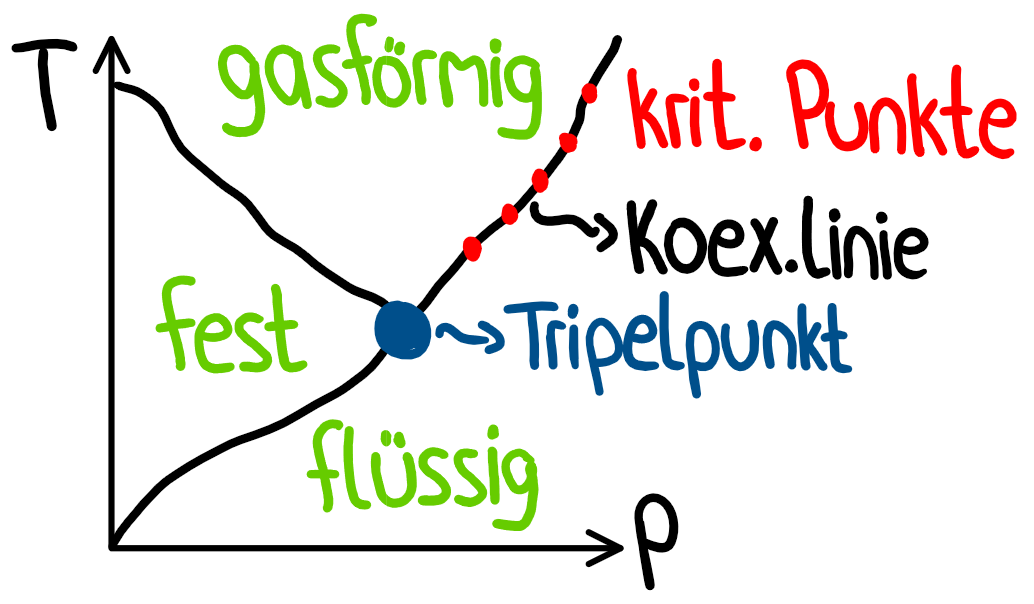
\includegraphics[width=0.5\textwidth,angle=0]{Bilder/phdia.png}
%\captionof{figure}{}\medskip
\label{fig:}
\end{center}



will punkte mit gleicher steigung verbinden bei maxwell-konstruktion (damit Übergang smooth; so sind diese flächen unter dem graphen jeweils gleich), was genau dem ersetzen des potentials mit konvexer hülle entspricht (allgemeinere formulierung)


kriegen bei kleinen volumina auch falsche ergebnisse, denn eigentlich hat man ja einen weiteren phasenübergang bei zusammendrücken von flüssigkeit (= einfrieren)

phasenregel von gibbs: flache stücke sind simplizes (dreiecke, tetraeder etc.; eindeutige zerlegung in extremalpunkte im ganzen inneren) -> jede gemischte phase lässt sich eindeutig in reine phasen zerlegen (wohl toll in skript von straumann)


\end{document}